% \begin{name}
% 	{GV biên soạn: Huỳnh Trí Thiện\\ GV phản biện: Nguyễn Trí Minh Tuấn}
% 	{TOÁN 10-KNTT-CS}
% \end{name}
%----------------NỘI DUNG BIÊN SOẠN
% \setcounter{chapter}{3}
% \chapter{VECTƠ}
\newpage
\setcounter{section}{09}
\section{Vectơ trong mặt phăng tọa độ}
\subsection{KIẾN THỨC TRỌNG TÂM}
\subsubsection{Tọa độ của vectơ}
\begin{khung4}{}
\immini{\begin{itemize}
		\item [\iconMT] Hệ trục tọa độ bao gồm 2 trục vuông góc nhau (hình vẽ), kí hiệu $(O,\overrightarrow{i},\overrightarrow{j})$ hay $Oxy$.
		\begin{itemize}
			\item  $O$ là gốc tọa độ;
			\item $Ox$ gọi là trục hoành; $Oy$ gọi là trục tung;
			\item $\overrightarrow{i}$, $\overrightarrow{j}$ là các vectơ đơn vị và $|\overrightarrow{i}|=|\overrightarrow{j}|=1$.
		\end{itemize}
		\item [\iconMT] Xét điểm $M$ trên trục $(O,\overrightarrow{i}, \overrightarrow{j})$, ta luôn có $\overrightarrow{OM}=x_0\overrightarrow{i}+y_0\overrightarrow{j}$. Khi đó $(x_0,y_0)$ là tọa độ của $M$ trên hệ trục đã cho.
	\end{itemize}
}{
	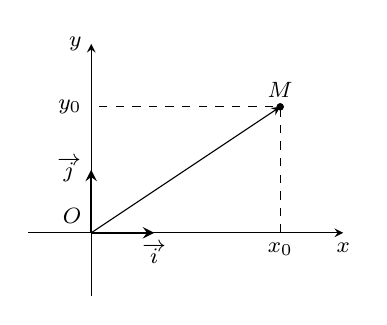
\begin{tikzpicture}[smooth,font=\footnotesize,scale=0.8,>=stealth]
		\draw[->] (-1,0)--(4,0) node [below]{$x$};
		\draw[->] (0,-1)--(0,3) node [left]{$y$};
		\draw[->,thick] (0,0)--(1,0) node [below]{$\overrightarrow{i}$};
		\draw[->,thick] (0,0)--(0,1) node [left]{$\overrightarrow{j}$};
		\draw (0,0) node[above left]{$O$};
		\draw[->] (0,0)--(3,2);
		\draw[dashed] (3,0)node [below]{$x_0$}--(3,2)node [above]{$M$}--(0,2)node [left]{$y_0$} ;
		\draw [fill=black] (3,2) circle (.05);
		%\node[below right] at (1.5,1.2){$\vec{u}$};
\end{tikzpicture}}
\end{khung4}
\begin{khung4}{}
\immini{\begin{itemize}
	\item [\iconMT] \indam{Định nghĩa:} Với mỗi vectơ $\vec{u}$ trên mặt phẳng $Oxy$, có duy nhất cặp số $(x_0;y_0)$ sao cho $\vec{u}=x_0\vec{i}+y_0\vec{j}$. Ta nói $\vec{u}$ có tọa độ là $(x_0;y_0)$ và viết $\vec{u}=(x_0;y_0)$ hoặc $\vec{u}(x_0;y_0)$.
	\item [\iconMT] \indam{Chú ý:}
	\begin{itemize}
		\item Tọa độ hai vectơ đơn vị là $\vec{i}=(1;0)$, $\vec{j}=(0;1)$.
		\item $\overrightarrow{u}(x;y)=\overrightarrow{v}(x';y')\Leftrightarrow \heva{&x=x'\\ & y=y'}$.
	\end{itemize}
\end{itemize}}{
		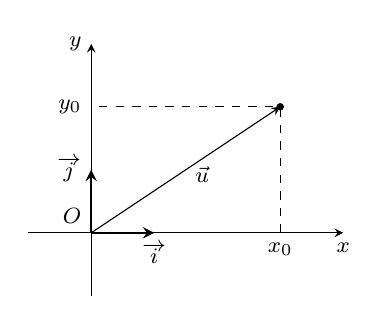
\begin{tikzpicture}[smooth,font=\footnotesize,scale=0.8,>=stealth]
		\draw[->] (-1,0)--(4,0) node [below]{$x$};
		\draw[->] (0,-1)--(0,3) node [left]{$y$};
		\draw[->,thick] (0,0)--(1,0) node [below]{$\overrightarrow{i}$};
		\draw[->,thick] (0,0)--(0,1) node [left]{$\overrightarrow{j}$};
		\draw (0,0) node[above left]{$O$};
		\draw[->] (0,0)--(3,2);
		\draw[dashed] (3,0)node [below]{$x_0$}--(3,2)--(0,2)node [left]{$y_0$} ;
		\draw [fill=black] (3,2) circle (.05);
		\node[below right] at (1.5,1.2){$\vec{u}$};
\end{tikzpicture}}
\end{khung4}
\begin{khung4}{}
	Hai vectơ bằng nhau khi và chỉ khi chúng có cùng toạ độ.
	$$ \overrightarrow{u}(x; y)=\overrightarrow{v}\left(x'; y'\right) \Leftrightarrow \heva{& x=x' \\& y=y'.} $$
\end{khung4}
\subsubsection{Biểu thức tọa độ của các phép toán vectơ}
\begin{khung4}{}
	Cho hai vectơ $\overrightarrow{u}=\left(x; y\right)$ và $\overrightarrow{v}=\left(x'; y'\right)$. Khi đó
	\begin{itemize}
		\item $\overrightarrow{u}+\overrightarrow{v}=\left(x+x'; y+y'\right)$.
		\item $\overrightarrow{u}-\overrightarrow{v}=\left(x-x'; y-y'\right)$.
		\item $k\overrightarrow{u}=\left(kx; ky\right)$, với $k \in \mathbb{R}$.
	\end{itemize}
\end{khung4}

\begin{khung4}{}
	\begin{itemize}
	\item Với vectơ $\overrightarrow{u}=\left(x; y\right)$, ta lấy điểm $M\left(x; y\right)$ thì $\overrightarrow{u}=\overrightarrow{OM}$. \\ Do đó, $\left|\overrightarrow{u}\right|=\left|\overrightarrow{OM}\right|=\sqrt{x^2+y^2}$.
	\item Vectơ $\overrightarrow{v}\left(x'; y'\right)$ cùng phương với vectơ $\overrightarrow{u}\left(x; y\right)\ne\overrightarrow{0}$ khi và chỉ khi tồn tại số $k$ sao cho $$x'=k\cdot x, y'=k\cdot y \left(\text{hay là } \dfrac{x'}{x}=\dfrac{y'}{y} \text{ nếu } xy\ne0\right).$$
	\end{itemize}
\end{khung4}
\begin{khung4}{}
	Cho ba điểm $A\left( x_A;y_A \right)$, $B\left( x_B;y_B\right)$ và $C\left( x_C;y_C\right)$. Khi đó
% \begin{tcolorbox}[colframe=cyan,colback=white,boxrule=0.2mm]
	\begin{listEX}[1]
		\item [\ding{172}] $\overrightarrow{AB}=\left( x_B-x_A;y_B-y_A\right)$ 
		\item [\ding{173}] Khoảng cách giữa hai điểm $A$, $B$ là $AB=\sqrt{\left( x_B-x_A\right)^2+\left(y_B-y_A\right)^2}$.
		\item [\ding{174}] Trung điểm $I$ của $AB$:	$x_I=\dfrac{x_A+x_B}{2}$ và $y_I=\dfrac{y_A+y_B}{2}$
		\item [\ding{175}] $G$ là trọng tâm tam giác $ABC$: 
		$x_G=\dfrac{x_A+x_B+x_C}{3}$ và $y_G=\dfrac{y_A+y_B+y_C}{3}$.
		\item [\ding{176}] $ABC$ là ba đỉnh của tam giác $\Leftrightarrow $ $\overrightarrow{AB}$ không cùng phương với $\overrightarrow{AC}$
\end{listEX}
% \end{tcolorbox}
\end{khung4}
\subsection{PHÂN LOẠI VÀ PHƯƠNG PHÁP GIẢI TOÁN}

\begin{dang}{Tọa độ vectơ}
	
\end{dang}

\begin{vd}
	Viết tọa độ của các vectơ sau
	\begin{tasks}(3)
		\task $\overrightarrow{a}=2\overrightarrow{i}+3\overrightarrow{j}$.
		\task $\overrightarrow{b}=\dfrac{1}{3}\overrightarrow{i}-5\overrightarrow{j}$.
		\task $\overrightarrow{c}=3\overrightarrow{i}$.
	\end{tasks}
\end{vd}
\dongcham{1}
\begin{vd}
	Cho $\overrightarrow{a}=(1;-2)$, $\overrightarrow{b}=(0;3)$. Tìm toạ độ của các vectơ sau
	\begin{tasks}(1)
		\task $\overrightarrow{x}=\overrightarrow{a}+\overrightarrow{b}$;\quad $\overrightarrow{y}=\overrightarrow{a}-\overrightarrow{b}$;\quad $\overrightarrow{z}=2\overrightarrow{a}-3\overrightarrow{b}$.
		\task $\overrightarrow{u}=3\overrightarrow{a}-2\overrightarrow{b}$;\quad $\overrightarrow{v}=2\overrightarrow{a}+\overrightarrow{b}$;\quad $\overrightarrow{w}=4\overrightarrow{a}-\dfrac{1}{2}\overrightarrow{b}$.
	\end{tasks}
\end{vd}
\dongcham{6}

\begin{vd}
	Cho $\overrightarrow{a}=(2;1)$, $\overrightarrow{b}=(3;4)$, $\overrightarrow{c}=(7;2)$.
	\begin{tasks}(1)
		\task Tìm tọa độ của vectơ $\overrightarrow{u}=2\overrightarrow{a}-3\,\overrightarrow{b}$.
		\task Tìm tọa độ của vectơ $\overrightarrow{x}$ sao cho $\overrightarrow{x}+\overrightarrow{a}=\overrightarrow{b}-\overrightarrow{c}$.
	\end{tasks}
\end{vd}
\dongcham{6}

\begin{vd}
	Cho $\overrightarrow{a}=(-2;0)$, $\overrightarrow{b}=(3;4)$, $\overrightarrow{c}=(7;2)$. Tính tọa độ vectơ
	\begin{tasks}(2)
		\task  $\overrightarrow{u}=2\overrightarrow{a}-4\overrightarrow{b}+\overrightarrow{c}$.
		\task $\overrightarrow{v}=-\overrightarrow{a}+\dfrac{1}{3}\cdot\overrightarrow{b}-\dfrac{1}{2}\cdot\overrightarrow{c}$.
	\end{tasks}
\end{vd}
\dongcham{6}

\begin{dang}{Hai vectơ cùng phương}
	 Cho hai vectơ $\overrightarrow{a}=\left( a_1;a_2 \right)$ và $\overrightarrow{b}=\left( b_1;b_2\right)$.  
	 \begin{itemize}
	 	\item [\iconMT] Điều kiện cần và đủ để $\overrightarrow{a}$ và $\overrightarrow{b} \ne \overrightarrow{0}$ cùng phương là $\exists k \in \mathbb{R} \colon \overrightarrow{a}=k\overrightarrow{b} \Leftrightarrow \heva{&a_1=kb_1\\&a_2=kb_2}$.
	 	\item [\iconMT] Nếu $b_1$ và $b_2$ khác $0$ thì $\overrightarrow{a}$ và $\overrightarrow{b} \ne \overrightarrow{0}$ cùng phương khi  $\dfrac{a_1}{b_1}=\dfrac{a_2}{b_2}$.
	 
	 \end{itemize}
\end{dang}

\begin{vd}
	Cặp vectơ nào sau đây cùng phương? cùng hướng? ngược hướng?
	\begin{tasks}(2)
		\task $\vec{a}=(1;2)$ và $\vec{b}=(2;4)$.
		\task $\vec{a}=(-3;2)$ và $\vec{b}=(1;2)$.
		\task $\vec{a}=(3;0)$ và $\vec{b}=(2;0)$.
		\task $\vec{a}=(4;-2)$ và $\vec{b}=(-2;1)$.
		\task $\vec{a}=(0;5)$ và $\vec{b}=(4;0)$.
		\task $\vec{a}=(0;2)$ và $\vec{b}=(0;-3)$.
	\end{tasks}
	
\end{vd}
\dongcham{6}

\begin{vd}
	Cho $\overrightarrow{a}=(2;1)$, $\overrightarrow{b}=(m^2-m;3)$. Tìm $m$ để hai vectơ $\overrightarrow{a}$ và $\overrightarrow{b}$ cùng phương.
\end{vd}
\dongcham{3}

\begin{vd}%[0H1G4-5]%
	Trong mặt phẳng tọa độ $Oxy$, cho $\vec{a}=(m;2)$, $\vec{b}=(1-m;m+4)$ (với $m$ là tham số). Tìm $m$ sao cho $2\vec{a}-3\vec{b}$ cùng phương với $\vec{c}=(4;-2)$.
	\loigiai{
		Ta có $\vec{d}=2\vec{a}-3\vec{b}=(5m-3;-3m-8)$. Hai vectơ $\vec{d}$, $\vec{c}$ cùng phương khi và chỉ khi $$(5m-3)\cdot (-2)=(-3m-8)\cdot 4\Leftrightarrow m=-19.$$
	}
\end{vd}
\dongcham{3}

\begin{dang}{Phân tích vectơ theo hai vectơ không cùng phương}
	Giả sử cần phân tích $\vec{u}=(u_1;u_2)$ theo hai vectơ không cùng phương $\vec{a}=(a_1;a_2)$ và $\vec{b}=(b_1;b_2)$. Ta thực hiện như sau:
	\begin{itemize}
		\item [$\bullet$] Giả sử $\vec{u} =m \cdot \vec{a} + n \cdot \vec{b}$ với $m,n \in \mathbb{R}$.
		\item [$\bullet$] Dùng điều kiện vectơ bằng nhau, ta được hệ
		$\heva{&u_1=m\cdot a_1 + n\cdot b_1\\&u_2=m\cdot a_2 + n\cdot b_2}.$
		\item [$\bullet$] Giải hệ trên tìm $m$ và $n$. Kết luận $\vec{u} =m \cdot \vec{a} + n \cdot \vec{b}$ với $m$, $n$ vừa tìm được.
	\end{itemize}
	
\end{dang}
\dongcham{5}

\begin{vd}
	Phân tích vectơ $\overrightarrow{u}$ theo hai vectơ $\overrightarrow{a}$ và $\overrightarrow{b}$, biết
	\begin{tasks}(2)
		\task $\overrightarrow{u}=(-4;7)$, $\overrightarrow{a}=(2;-1)$, $\overrightarrow{b}=(-3;4)$.
		\task $\overrightarrow{u}=(-1;3)$, $\overrightarrow{a}=(1;1)$, $\overrightarrow{b}=(2;3)$.
		\task $\overrightarrow{u}=(-1;3)$, $\overrightarrow{a}=(2;1)$, $\overrightarrow{b}=(3;2)$.
		\task $\overrightarrow{u}=2\overrightarrow{i}-3\overrightarrow{j}$, $\overrightarrow{a}=(1;1)$, $\overrightarrow{b}=(2;3)$.
	\end{tasks}
\end{vd}


\begin{dang}{Tọa độ điểm}
	Các bài toán thường gặp
	\begin{listEX}[1]
		\item [\ding{172}] Tìm điểm $I$ là trung điểm của đoạn thẳng cho trước.
		\item [\ding{173}] Tìm điểm $G$ là trọng tâm của tam giác cho trước.
		\item [\ding{174}] Tìm điểm $M$ thỏa mãn một đẳng thức vectơ.
		\item [\ding{175}] Tìm điểm $M$ trên $Ox$ hoặc $Oy$ cùng với hai điểm cho trước thẳng hàng.
		\item [\ding{176}] Tìm điểm $D$ sao cho tứ giác $ABCD$ là hình bình hành.
	\end{listEX}
\end{dang}
\begin{vd}
	Trên mặt phẳng $Oxy$ cho 2 điểm $A\left( -2;-2 \right)$ và $B\left( 5;-4 \right)$.
	Tìm tọa độ trọng tâm của tam giác $OAB$.
	Tìm tọa độ điểm $C$ sao cho tam giác $ABC$ có trọng tâm là điểm $G\left( 2;0 \right)$.
\end{vd}
\dongcham{6}

\begin{vd}
	Cho $A\left( -3;4 \right),B\left( 1;1 \right),C\left( 5;5 \right)$.
	\begin{tasks}(1)
		\task Tìm điểm $D$ sao cho $A$ là trung điểm $BD$.
		\task Tìm điểm $E$ trên trục $Ox$ sao cho $A,B,E$ thẳng hàng.
	\end{tasks}
\end{vd}
\dongcham{6}

\begin{vd}
	Cho ba điểm $A(-3;4)$, $B(1;1)$, $C(2;-5)$.
	\begin{tasks}(1)
		\task Chứng minh ba điểm $A$, $B$, $C$ không thẳng hàng.
		\task Gọi $M$, $N$, $P$ lần lượt là trung điểm của $AB$, $BC$, $CA$. Tìm tọa độ $M$, $N$, $P$.
		\task Tìm tọa độ điểm $D$ sao cho $ABCD$ là hình bình hành.
		\task Tìm tọa độ điểm $E$ trên trục tung sao cho $\overrightarrow{AE}$ và $\overrightarrow{BC}$ cùng phương.
	\end{tasks}
\end{vd}
\dongcham{8}

\begin{vd}
	Cho ba điểm $A(1;1)$, $B(2;3)$, $ C(0;5)$.
	\begin{tasks}(1)
		\task Chứng minh $A$, $B$, $C$ là 3 đỉnh của một tam giác. Tìm tọa độ trọng tâm của tam giác $ABC$. 
		\task Tìm tọa độ điểm $K$ sao cho tứ giác $ABKC$ là hình bình hành.
		\task Tìm tọa độ điểm $D$ trên trục hoành sao cho $ABCD$ là hình thang.
	\end{tasks}
\end{vd}
\dongcham{8}

\begin{vd}
	Cho hai điểm $A(-2;2)$, $I(3;1)$ Tìm tọa độ điểm $A'$ đối xứng với $A$ qua $I$.
\end{vd}
\dongcham{3}

\begin{vd}
	Cho tam giác $ABC$ có trọng tâm $G$. Biết $A(1;1)$, $B(-3;2)$, $G(2;3)$. Tìm tọa độ điểm $C$.
\end{vd}
\dongcham{3}

\begin{vd}
	Cho tam giác $ABC$. Biết các điểm $M(1;1)$, $N(2;3)$, $P(0;4)$ lần lượt là trung điểm các cạnh $AB$, $BC$, $CA$.
	\begin{tasks}(1)
		\task Tìm tọa độ các đỉnh $A$, $B$, $C$.
		\task Tìm tọa độ trọng tâm $G$ của tam giác $ABC$.
	\end{tasks}
\end{vd}
\dongcham{6}

\begin{vd}
	Cho tam giác $ABC$. Các điểm $M(1; 0)$, $N(2; 2)$, $P(-1; 3)$ lần lượt là trung điểm các cạnh $BC$, $CA$, $AB$. Tìm tọa độ các đỉnh của tam giác $ABC$.
\end{vd}
\dongcham{6}
\begin{vd}
	Cho ba điểm $A(-1; 2)$, $B (3; -4)$, $C(5; 0)$. Tìm tọa độ điểm $D$ nếu biết
	\begin{tasks}(1)
		\task $\overrightarrow{AD}-2\overrightarrow{BD}+3\overrightarrow{CD}=\overrightarrow{0}$.
		\task $\overrightarrow{AD}-2\overrightarrow{AB}=2\overrightarrow{BD}+\overrightarrow{BC}$.
		\task tứ giác $ABCD$ hình bình hành.
		\task tứ giác $ABCD$ hình thang có hai đáy là $BC$, $AD$ với $BC = 2AD$.
	\end{tasks}
\end{vd}
\dongcham{8}

\begin{vd}
	Cho hai điểm $I(1; -3)$, $J(-2; 4)$ chia đọan $AB$ thành ba đọan bằng nhau $AI = IJ = JB$.
	\begin{tasks}(1)
		\task Tìm tọa độ của $A$, $B$.
		\task Tìm tọa độ của điểm $I'$ đối xứng với $I$ qua $B$.
		\task Tìm tọa độ của $C$, $D$ biết $ABCD$ hình bình hành tâm $K(5, -6)$.
	\end{tasks}
\end{vd}
\dongcham{8}

\begin{vd}
	Cho ba điểm $A\left( 1;1 \right)$, $B\left( 3;2 \right)$ và $C\left( m+4;2m+1 \right)$ . Tìm $m$ để ba điểm $A$, $B$, $C$ thẳng hàng.
\end{vd}
\dongcham{4}

\begin{vd}
	Cho hai điểm $A\left( 3;4 \right),B\left( 2;5 \right)$ . Tìm $x$ để điểm $C\left( -7;x \right)$ thuộc đường thẳng $AB$.
\end{vd}
\dongcham{4}

\begin{vd}
	Trong mặt phẳng tọa độ $Oxy$, cho hình bình hành $ABCF$ có $A(-4;1)$, $B(2;4)$, $C(2;-2)$. Gọi $M$ là điểm nằm trên đoạn $FB$ sao cho $2FM=3MB$. Tính tọa độ vectơ $\vec{MB}$.
	\loigiai{
		\immini{Ta có $\vec{BA}=(-6;-3),\vec{BC}=(0;-6)$.\\
			Từ giả thiết có \begin{align*}
				\vec{MB}&=-\dfrac{2}{5}\vec{BF}\\
				&=-\dfrac{2}{5}\left(\vec{BA}+\vec{BC}\right)\\
				&=-\dfrac{2}{5}(-6+0;-3-6)\\
				&=\left(\dfrac{12}{5};\dfrac{18}{5}\right).
		\end{align*}}
		{\begin{tikzpicture}[scale=0.6]
				\tkzInit[ymin=-1,ymax=10,xmin=-1,xmax=15]
				\tkzSetUpPoint[color=black,fill=white,size=6]
				\tkzDefPoints{-4/1/A,2/4/B,2/-2/C}
				\tkzDefPointBy[translation=from B to C](A)\tkzGetPoint{F}
				\tkzDefPointBy[homothety=center B ratio 0.4](F)\tkzGetPoint{M}
				\tkzDrawSegments(A,B B,C C,F F,A F,B)
				\tkzDrawPoints(A,B,C,F,M)
				\tkzLabelPoints[left](A,B,F,M)
				\tkzLabelPoints[below](C)
		\end{tikzpicture}}
	}
\end{vd}
\dongcham{5}

\begin{dang}{Tính độ dài đoạn thẳng} 
	Chú ý các công thức sau:
	\begin{itemize}
		\item [$\bullet$] $\overrightarrow{AB}=\left( x_B-x_A;y_B-y_A\right)$ 
		\item [$\bullet$] Khoảng cách giữa hai điểm $A$, $B$ là $AB=\sqrt{\left( x_B-x_A\right)^2+\left(y_B-y_A\right)^2}$.
	\end{itemize}
\end{dang}

\begin{vd}
	Trong mặt phẳng $Oxy$, cho tam giác $ABC$ với $A(1;4)$, $B(2;2)$, $C(8;5)$.
	\begin{tasks}(1)
		\task Tính độ dài các cạnh của tam giác $ABC$. Chứng tỏ tam giác $ABC$ vuông tại $B$.
		\task Tính chu vị và diện tích tam giác $ABC$ (kết quả làm tròn đến 2 chữ số thập phân).
	\end{tasks}
\end{vd}
\dongcham{5}

\begin{vd}
	Trong mặt phẳng $Oxy$, cho $A(-2;2)$, $B\left(\dfrac{5}{2};2+\dfrac{3\sqrt{3}}{2} \right)$, $C\left(\dfrac{5}{2};2-\dfrac{3\sqrt{3}}{2} \right)$
	\begin{tasks}(1)
		\task Tính độ dài các cạnh của tam giác $ABC$. Chứng tỏ tam giác $ABC$ đều.
		\task Tính diện tích tam giác $ABC$ (kết quả làm tròn đến 2 chữ số thập phân).
	\end{tasks}
\end{vd}
\dongcham{5}

\begin{vd}
	Trong mặt phẳng $Oxy$, cho $\vec{OA}=(1;3)$ và $B(7;6)$.
	\begin{tasks}(1)
		\task Tính độ dài đoạn $OA$.
		\task Tìm điểm $M$ trên $Ox$ sao cho tam giác $ABM$ cân tại $B$.
	\end{tasks}
\end{vd}
\dongcham{5}

\begin{vd}
	Trong mặt phẳng $Oxy$, cho điểm $A(2;1)$ và $\vec{AB}=(1;3)$.
	\begin{tasks}(1)
		\task Tìm toạ độ điểm $A$.
		\task Tìm điểm $M$ trên $Oy$ sao cho tam giác $ABM$ cân tại $B$.
	\end{tasks}
\end{vd}
\dongcham{6}

\subsection{VẬN DỤNG, THỰC TIỄN}
\begin{dang}{Tọa độ hóa một số mô hình hình học}
\end{dang}
\begin{vd}
	Cho tam giác đều $ABC$ cạnh $a$. Chọn hệ trục tọa độ $Oxy$, trong đó $O$ là trung điểm $BC$, $Ox$ cùng hướng với $\overrightarrow{OC}$, $Oy$ cùng hướng $\overrightarrow{OA}$.
	\begin{tasks}(1)
		\task Tính tọa độ của các đỉnh của tam giác $ABC$.
		\task Tìm tọa độ trung điểm $E$ của $AC$.
		\task Tìm tọa độ tâm đường tròn ngoại tiếp tam giác $ABC$.
	\end{tasks}
\end{vd}
\dongcham{10}

\begin{vd}%[0H1G4-3]%
	Cho hình bình hành $ABCD$ có $AD=4$, chiều cao ứng với cạnh $AD$ bằng $3$, góc $\widehat{BAD}=60^\circ$. Chọn hệ trục tọa độ $(A;\overrightarrow i, \overrightarrow j)$ với $\overrightarrow i =(1;0)$ và $\overrightarrow j =(0;1)$ sao cho $\overrightarrow i$ và $\overrightarrow{AD}$ cùng hướng, $y_B>0$. Tìm tọa độ đỉnh $C$ của hình bình hành đã cho.
	\loigiai{
		\immini{
			Bài toán được mô tả như hình vẽ.\\
			Từ giả thiết, ta suy ra $BH=3$, $AB=2\sqrt{3}$, $AH=\sqrt{3}$. Do đó, $B(\sqrt3; 3)$.\\
			Khi đó, ta tính được $$\overrightarrow{AC}=\overrightarrow{AB}+\overrightarrow{AD}=(\sqrt3; 3)+(4; 0)=(4+\sqrt3; 3).$$
			Vậy, tọa độ của đỉnh $C$ là $(4+\sqrt{3};3)$.
		}
		{
		\begin{tikzpicture}[smooth,samples=300,scale=0.8,>=stealth,font=\footnotesize]
			\draw[->] (-0.8,0)--(6.5,0) node[below]{$x$};
			\draw[->] (0,-0.5)--(0,3.5) node[right]{$y$};
			\draw[->] (0,0)--(1,0) node[below]{$\vec{i}$};
			\draw[->] (0,0)--(0,1) node[left]{$\vec{j}$};
			\tkzDefPoints{0/0/A,1.5/2/B,5.5/2/C,4/0/D,1.5/0/H}
			\tkzDrawPolygon(A,B,C,D)
			\tkzDrawSegments(B,H)
			\tkzDrawPoints[size=2,fill=black](A,B,C,D,H)
			\tkzLabelPoints[below](D,H)
			\tkzLabelPoints[below left](A)
			\tkzLabelPoints[above](B,C)
			
		\end{tikzpicture}
		}
	}
\end{vd}
\dongcham{6}

\begin{vd}
	Để kéo một đường dây điện băng qua một hồ hình chữ nhật $ABCD$ với độ dài $AB=200$m, $AD=180$m, người ta định làm 4 cột điện liên tiếp cách đều nhau, cột thứ nhất nằm trên bờ $AB$ và cách đỉnh $A$ khoảng cách 20 m, cột thứ tư nằm trên bờ $CD$ và cách đỉnh $C$ khoảng 30 m. Tính khoảng cách từ vị trí các cột thứ hai, thứ ba đến các bờ $AB$, $CD$.
	\loigiai{
	\immini{
	Chọn hệ trục tọa độ $Oxy$ như hình vẽ. Khi đó $A(0;0)$,  $B(200;0)$, $C(200;180)$, $D(0;180)$. Các vị trí trồng cột điện lần lượt là $C_1$, $C_2$, $C_3$, $C_4$.\\
	Tọa độ $C_1(20;0)$ và $C_4(170;180)$. 
\begin{itemize}
	\item [$\bullet$] Ta có $\vec{C_1C_2}=\dfrac{1}{3}\vec{C_1C_4}$. Từ đây giải được $C_2(70;60)$. Suy ra khoảng cách từ cột thứ hai đến bờ $AB$ là 60 m, đến bờ $CD$ là $180 - 60 =120$m.
	\item [$\bullet$] Tương tự ta có $\vec{C_1C_3}=\dfrac{2}{3}\vec{C_1C_4}$. Từ đây giải được $C_3(120;120)$. Suy ra khoảng cách từ cột thứ ba đến bờ $AB$ là 120 m, đến bờ $CD$ là $180 - 120 =60$m.
\end{itemize}}{
	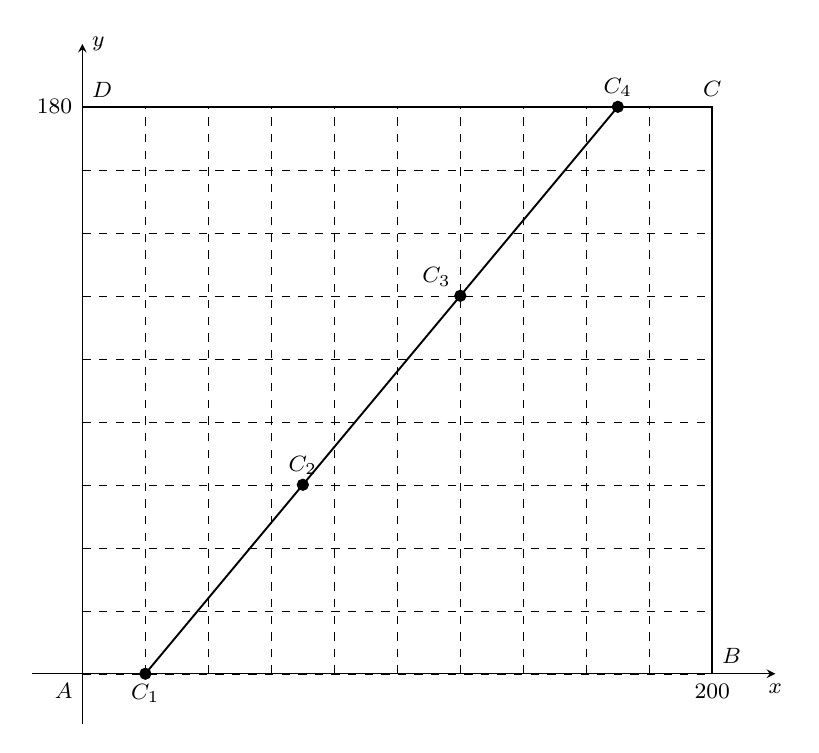
\begin{tikzpicture}[smooth,samples=300,scale=0.8,>=stealth,font=\footnotesize]
		\draw[->] (-0.8,0)--(11,0) node[below]{$x$};
		\draw[->] (0,-0.8)--(0,10) node[right]{$y$};
		\draw[line width=0.1pt,dashed] (0,0) grid (10,9);
		\draw (0,0) node[below left]{$A$};
		\draw[line width=0.7pt] (1,0)node[below]{$C_1$}--(8.5,9)node[above]{$C_4$};
		\draw[line width=0.7pt] (10,0)node[below]{$200$}--(10,9)node[above]{$C$}--(0,9)node[left]{$180$};
		\draw[fill=black] (1,0) circle(2.5pt) (3.5,3) circle(2.5pt) (6,6) circle(2.5pt) (8.5,9) circle(2.5pt);
		\node[above] at (3.5,3) {$C_2$};
		\node[above left] at (6,6) {$C_3$};
		\node[above right] at (10,0) {$B$};
		\node[above right] at (0,9) {$D$};
\end{tikzpicture}}
}
\end{vd}
\dongcham{10}

\begin{vd}%[0H9H1-6]
	\immini{Một trò chơi trên máy tính đang mô phỏng một vùng biển có hai hòn đảo nhỏ có tọa độ $B\left(50;30\right)$, $C\left(32;-32\right)$. Một con tàu đang neo đậu tại điểm $A\left(-10; 20\right)$. Cho biết một đơn vị trên trục tọa độ tương ứng với $1$ km. Tính tổng khoảng cách từ con tàu đến mỗi hòn đảo (\textit{làm tròn kết quả đến hàng phần mười}).}
	{
	\begin{tikzpicture}[scale=0.06, >=stealth,font=\footnotesize]
		% --- Hệ trục tọa độ ---
		\draw[->] (-25,0) -- (65,0) node[below]{$x$};
		\draw[->] (0,-45) -- (0,45) node[left]{$y$};
		\node[below right ] at (0,0) {$O$};
		% --- Các điểm ---
		\coordinate (A) at (-10,20);
		\coordinate (B) at (50,30);
		\coordinate (C) at (32,-32); % Đã sửa tọa độ
		% --- Vẽ đoạn thẳng nối ---
		\draw[thick] (A) -- (B);
		\draw[thick] (A) -- (C);
		% --- Minh họa Con tàu (A) ---
		\fill[blue!70] (A) circle (10pt);
		% Vẽ hình dáng tàu đơn giản
		\draw[fill=white, thick] ($(A)+(-4,2)$) -- ($(A)+(4,2)$) -- ($(A)+(3,-1)$) -- ($(A)+(-3,-1)$) -- cycle;
		\draw[thick] ($(A)+(0,2)$) -- ($(A)+(0,5)$) -- ($(A)+(2,3.5)$) -- cycle;
		\node[below left, xshift=-2mm] at (A) {$A$};
		% --- Minh họa Đảo (B) ---
		\fill[green!60!black] (B) circle (10pt);
		\draw[fill=yellow!80!black] ($(B)+(-5,-2)$) to[out=30,in=150] ($(B)+(5,-2)$) -- cycle;
		\draw[thick, brown] (B) -- ($(B)+(0,5)$);
		\draw[thick, green!50!black] ($(B)+(0,5)$) to[out=45,in=135] ($(B)+(3,3)$);
		\draw[thick, green!50!black] ($(B)+(0,5)$) to[out=135,in=45] ($(B)+(-3,3)$);
		\node[above right, xshift=2mm] at (B) {$B$};
		% --- Minh họa Đảo (C) ---
		\fill[green!60!black] (C) circle (10pt);
		\draw[fill=yellow!80!black] ($(C)+(-5,-2)$) to[out=30,in=150] ($(C)+(5,-2)$) -- cycle;
		\draw[thick, brown] (C) -- ($(C)+(0,5)$);
		\draw[thick, green!50!black] ($(C)+(0,5)$) to[out=45,in=135] ($(C)+(3,3)$);
		\draw[thick, green!50!black] ($(C)+(0,5)$) to[out=135,in=45] ($(C)+(-3,3)$);
		\node[below right, xshift= 3mm ] at (C) {$C$};
		% --- Gióng tọa độ (nét đứt) ---
		\draw[dashed, gray] (A) -- (-10,0) node[below, black]{$-10$};
		\draw[dashed, gray] (A) -- (0,20) node[right, black]{$20$};
		\draw[dashed, gray] (B) -- (50,0) node[below, black]{$50$};
		\draw[dashed, gray] (B) -- (0,30) node[left, black]{$30$};
		\draw[dashed, gray] (C) -- (32,0) node[above, black]{$32$};
		\draw[dashed, gray] (C) -- (0,-32) node[left, black]{$-32$};
	\end{tikzpicture}
	}
\loigiai{
	Vì con tàu đang neo đậu tại điểm $A\left(-10;20\right)$ và hòn đảo $B\left(50;30\right)$ nên khoảng cách từ con tàu đến hòn đảo $B$ là
	\[ AB = \sqrt{\left[50-\left(-10\right)\right]^2 + \left(30-20\right)^2} = \sqrt{60^2 + 10^2} = \sqrt{3700} \approx 60{,}8\,\text{km}. \]
	Vì con tàu đang neo đậu tại điểm $A\left(-10;20\right)$ và hòn đảo $C\left(32;-32\right)$ nên khoảng cách từ con tàu đến hòn đảo $C$ là
	\[ AC = \sqrt{\left[32-\left(-10\right)\right]^2 + \left(-32-20\right)^2} = \sqrt{42^2 + \left(-52\right)^2} = \sqrt{1764+2704} = \sqrt{4468} \approx 66{,}8\,\text{km}. \]
	Tổng khoảng cách từ con tàu đến mỗi hòn đảo là
	\[ AB + AC \approx 60{,}8 + 66{,}8 = 127{,}6\,\text{km}. \]
	}
\end{vd}
\dongcham{8}

\begin{vd}%[0H9V1-6]
	\immini{Trong hình bàn cờ vua dưới đây, quân mã đang ở vị trí có toạ độ $\left(1; 2\right)$. Hỏi sau một nước đi, quân mã có thể đến những vị trí nào?
	}{
	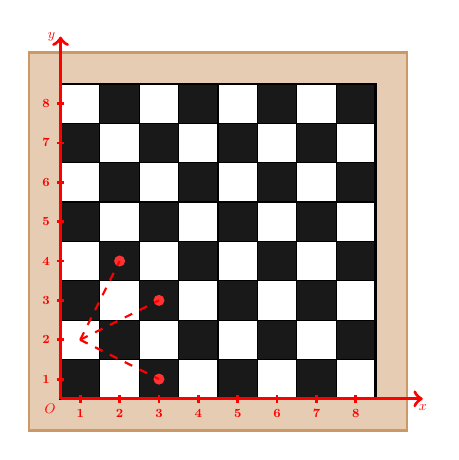
\begin{tikzpicture}[scale=0.5, transform shape]
		% 1. VẼ VIỀN GỖ (Border)
		\fill[brown!40] (-0.8,-0.8) rectangle (8.8,8.8);
		\draw[brown!80, line width=1pt] (-0.8,-0.8) rectangle (8.8,8.8);
		% 2. VẼ BÀN CỜ
		% Quy tắc: Ô (1;1) là ô ĐEN.
		% Do (1;1) tương ứng x=0.5, y=0.5 (hàng 1 cột 1).
		% TikZ loop x=0, y=0 -> x+y=0 (chẵn). Nếu chẵn là đen thì (0,0) đen.
		\foreach \x in {0,...,7} \foreach \y in {0,...,7} {
		\pgfmathparse{mod(\x+\y,2) == 0 ? 1 : 0}
		\ifnum\pgfmathresult=1
		\fill[black!90] (\x,\y) rectangle ++(1,1); % Ô đen
		\else
		\fill[white] (\x,\y) rectangle ++(1,1);   % Ô trắng
		\fi
		}
		\draw[black, thin] (0,0) grid (8,8);
		\draw[black, thick] (0,0) rectangle (8,8);
		% 3. VẼ HỆ TRỤC TOẠ ĐỘ
		% Trục nằm sát viền bàn cờ
		\draw[->, red, line width=1.2pt] (0,0) -- (9.2,0) node[below] {$x$};
		\draw[->, red, line width=1.2pt] (0,0) -- (0,9.2) node[left] {$y$};
		\node[red, below left, font=\bfseries] at (0,0) {$O$};
		% 4. ĐÁNH SỐ VÀ VẠCH CHIA (QUAN TRỌNG: CĂN GIỮA TÂM Ô)
		% Số 1 ứng với tâm ô đầu tiên (x=0.5)
		\foreach \i in {1,...,8} {
		% Vạch chia trục hoành (nằm tại vị trí \i - 0.5)
		\draw[red, line width=1pt] (\i-0.5, 0.1) -- (\i-0.5, -0.1);
		\node[red, below, font=\small\bfseries] at (\i-0.5, -0.15) {\i};
		% Vạch chia trục tung (nằm tại vị trí \i - 0.5)
		\draw[red, line width=1pt] (0.1, \i-0.5) -- (-0.1, \i-0.5);
		\node[red, left, font=\small\bfseries] at (-0.15, \i-0.5) {\i};
		}
		% 5. QUÂN MÃ VÀ ĐIỂM ĐẾN (VẼ TẠI TÂM Ô)
		% Quân mã ở (1;2) -> Tâm ô là (0.5, 1.5)
		\node[font=\fontsize{22}{0}\selectfont, text=white] at (0.5, 1.5) {\textbf{\textit{M}}};
		% Điểm đến (2;4) -> Tâm (1.5, 3.5)
		\fill[red!80] (1.5, 3.5) circle (4pt);
		% Điểm đến (3;3) -> Tâm (2.5, 2.5)
		\fill[red!80] (2.5, 2.5) circle (4pt);
		% Điểm đến (3;1) -> Tâm (2.5, 0.5)
		\fill[red!80] (2.5, 0.5) circle (4pt);
		% Đường nối đứt nét
		\draw[dashed, red, thick] (0.5, 1.5) -- (1.5, 3.5);
		\draw[dashed, red, thick] (0.5, 1.5) -- (2.5, 2.5);
		\draw[dashed, red, thick] (0.5, 1.5) -- (2.5, 0.5);
	\end{tikzpicture}
	}
\loigiai{
	Quân mã đang ở vị trí $M(1; 2)$. Theo quy tắc di chuyển hình chữ L trên bàn cờ vua, quân mã có thể di chuyển đến các vị trí:
	\begin{itemize}
		\item Sang phải 1 ô, lên trên 2 ô $\Rightarrow (1+1; 2+2) = (2; 4)$.
		\item Sang phải 2 ô, lên trên 1 ô $\Rightarrow (1+2; 2+1) = (3; 3)$.
		\item Sang phải 2 ô, xuống dưới 1 ô $\Rightarrow (1+2; 2-1) = (3; 1)$.
	\end{itemize}
	Vậy quân mã có thể đến các vị trí có toạ độ: $(2; 4)$, $(3; 3)$ và $(3; 1)$.
	}
\end{vd}
\dongcham{6}

\begin{dang}{Một số bài toán liên quan đến max - min}
	
\end{dang}

\begin{vd}%[0H1K4-3]%
	Trong mặt phẳng tọa độ $Oxy$, cho tam giác $ABC$ có $A(2;2)$, $B(4;2)$, $C(3;1)$. Tìm tọa độ điểm $M$ thỏa mãn $\vec{MA}-\vec{MB}+\vec{MC}=\vec{0}$.
	\loigiai{
		Ta có
		$$\vec{MA}-\vec{MB}+\vec{MC}=\vec{0} \Leftrightarrow \vec{OM} = \vec{OA}-\vec{OB}+\vec{OC}
		\Rightarrow\heva{& x_M=x_A-x_B+x_C=1\\&y_M=y_A-y_B+y_C=1}\Rightarrow M(1;1).$$
	}
\end{vd}
\dongcham{6}

\begin{vd}%[0H1G4-3]%
	Trong mặt phẳng tọa độ $Oxy$, cho $A(-4;5)$, $B(-2;1)$. Tìm tọa độ của điểm $M$ trên trục tung sao cho $\left|\overrightarrow{MA}+\overrightarrow{MB}\right|$ ngắn nhất.
	\loigiai{
		Gọi $M(x;y) \in Oy \Rightarrow M(0;y)$.\\
		Ta có: $\heva{&\overrightarrow{MA}=(-4;5-y) \\& \overrightarrow{MB}=(-2;1-y)} \Rightarrow \overrightarrow{MA}+\overrightarrow{MB}=(-6;6-2y)$.\\
		$\Rightarrow \left|\overrightarrow{MA}+\overrightarrow{MB}\right|=\sqrt{72-24y+4y^2}=\sqrt{(2y-6)^2+36} \geq 6$.\\
		$\left|\overrightarrow{MA}+\overrightarrow{MB}\right|$ ngắn nhất là $6$. Dấu “=” xảy ra khi: $2y-6=0 \Leftrightarrow y=3$.\\
		Vậy $M(0;3)$.}
\end{vd}
\dongcham{8}

\begin{vd}%[0H1G4-3]%
	Trong mặt phẳng tọa độ $Oxy$, cho ba điểm $A(1;0)$, $B(0;5)$ và $C(-3;-5)$. Tìm tọa độ điểm $M$ thuộc trục $Oy$ sao cho $\left|3\overrightarrow{MA}-2\overrightarrow{MB}+4\overrightarrow{MC}\right|$ đạt giá trị nhỏ nhất.
	\loigiai{
		Gọi $I(a;b)$ là điểm thỏa mãn: $3\overrightarrow{IA}-2\overrightarrow{IB}+4\overrightarrow{IC}=\overrightarrow{0}$ \\
		Ta có: $3\overrightarrow{IA}-2\overrightarrow{IB}+4\overrightarrow{IC}=\overrightarrow{0}$ $ \Leftrightarrow 5\overrightarrow{IA}=2\overrightarrow{AB}-4\overrightarrow{AC}$ $ \Leftrightarrow \left\{\begin{aligned}
			&a=-\dfrac{9}{5}\\
			&b=-6\\
		\end{aligned}\right. $ $ \Rightarrow I\left(-\dfrac{9}{5};-6\right)$ \\
		Khi đó $\left|3\overrightarrow{MA}-2\overrightarrow{MB}+4\overrightarrow{MC}\right|$ $=\left|3\overrightarrow{IA}-2\overrightarrow{IB}+4\overrightarrow{IC}-5\overrightarrow{IM}\right|$ $=\left|\overrightarrow{0}-5\overrightarrow{IM}\right|$ $=5IM$ \\
		Do đó: $\left|3\overrightarrow{MA}-2\overrightarrow{MB}+4\overrightarrow{MC}\right|$ nhỏ nhất khi $IM$ ngắn nhất. Suy ra $M$ là hình chiếu vuông góc của $I\left(-\dfrac{9}{5};-6\right)$ trên $Oy$ $ \Rightarrow M(0;-6)$.}
\end{vd}
\dongcham{10}

\begin{vd}%[0H1G4-3]%
	Trong mặt phẳng tọa độ $ Oxy$, cho $ A(1;0)$, $ B(0;3)$, $ C(-3;-5)$. Tìm tọa độ điểm $ M$ thuộc trục $ Ox$ sao cho $\left|2\vec{MA}-3\vec{MB}+2\vec{MC}\right|$ nhỏ nhất.
	\loigiai{
		$M\in Ox\Rightarrow M(x;0)$.\\
		Ta có: $\vv{MA}=(1-x;0), \vv{MB}=(-x;3),\vv{MC}=(-3-x;-5)$.\\
		Suy ra: $2\vec{MA}-3\vec{MB}+2\vec{MC}=(-x-4;-19)$.\\
		Khi đó: $\left|2\vec{MA}-3\vec{MB}+2\vec{MC}\right|=\sqrt{(x+4)^2+19^2}\geq 19$.\\
		Do đó: $\left|2\vec{MA}-3\vec{MB}+2\vec{MC}\right|$ nhỏ nhất khi $x+4=0\Leftrightarrow x=-4$.\\
		Vậy $M(-4;0)$.
	}
\end{vd}
\dongcham{8}

\begin{vd}%[0H1G4-5]%
	Trong mặt phẳng tọa độ $Oxy$, cho hai điểm $A(-3;1)$, $B(-5;5)$. Tìm tọa độ điểm $M$ trên trục $Oy$ sao cho $|MA-MB|$ lớn nhất.
	\loigiai{
		Ta có $A$,$B$ nằm cùng phía đối với $Oy$ và $|MA-MB| \leq AB$. Do đó $|MA-MB|$ lớn nhất $\Leftrightarrow |MA-MB|=AB \Leftrightarrow A,B,M$ thẳng hàng.\\
		Gọi $M(0; t)$. Ta tính được $\vec{AB}=(-2; 4), \vec{AM}=(3; t-1).$ Do $A, B, M$ thẳng hàng nên $\dfrac3{-2}=\dfrac{t-1}4\Leftrightarrow t=-5$. Vậy $M(0;-5)$.
	}
\end{vd}
\dongcham{6}

\begin{vd}%[1261-1280 Sỹ Trường]%[0H1K4-5]%
	Trong mặt phẳng tọa độ $Oxy$, cho $M$ thuộc trục $Ox$ và $A(4; 1), B(1; 3)$. Tìm giá trị nhỏ nhất của biểu thức $T = MA + MB$.
	\loigiai
	{
		\immini{Ta có $A(4; 1), B(1; 3)$ nằm về cùng một phía đối với trục $Ox$.
			\\ Gọi $C$ đối xứng với $A$ qua trục $Ox$ suy ra $C(4; -1)$.
			\\ Với mọi điểm $M$ thuộc trục $Ox$ ta có $T= MA+MB = MC + MB \geq BC = 5$.}
		{\begin{tikzpicture}[>=stealth,scale=1, line join = round, line cap = round]
				\draw[->,line width = 1pt] (-1,0)--(0,0) node[below right]{$O$}--(5,0) node[below]{$x$};
				\draw[->,line width = 1pt] (0,-1.5) --(0,4) node[right]{$y$};
				\tikzset{label style/.style={font=\footnotesize}}
				\tkzDefPoints{4/1/A,1/3/B,4/-1/C,2/0/M}
				\tkzDrawSegments(M,A M,B M,C B,C)
				\tkzDrawSegments[dashed](A,C)
				\tkzDrawPoints(A,B,C,M)
				\tkzLabelPoints[left](B)
				\tkzLabelPoints[right](A,C)
				\tkzLabelPoints[below](M)
	\end{tikzpicture}}}
\end{vd}
\dongcham{6}

\subsection{BÀI TẬP RÈN LUYỆN}
\ind{PHẦN I.} \inden{Câu trắc nghiệm nhiều phương án lựa chọn. Mỗi câu hỏi học sinh chỉ chọn một phương án.}
\setcounter{ex}{0}
\Opensolutionfile{ans}[ans/ans-vec-to-oxy]
% Câu 1
\begin{ex}%[0H9N1-1]%[Huỳnh Trí Thiện]
	Trong hệ trục tọa độ $Oxy$, tọa độ của vectơ $\overrightarrow{a} = 8\overrightarrow{j} - 3\overrightarrow{i}$ bằng
	\choice
	{\True $\overrightarrow{a} = \left(-3; 8\right)$}
	{$\overrightarrow{a} = \left(3; -8\right)$}
	{$\overrightarrow{a} = \left(8; 3\right)$}
	{$\overrightarrow{a} = \left(8; -3\right)$}
\loigiai{
	Ta có $\overrightarrow{a} = 8\overrightarrow{j} - 3\overrightarrow{i} = -3\overrightarrow{i} + 8\overrightarrow{j} \Rightarrow \overrightarrow{a} = \left(-3; 8\right)$.
	}
\end{ex}
% Câu 2
\begin{ex}%[0H9N1-3]%[Huỳnh Trí Thiện]
	Trong mặt phẳng $Oxy$, cho hai điểm $B\left(-1; 3\right)$ và $C\left(3; 1\right)$. Độ dài vectơ $\overrightarrow{BC}$ bằng bao nhiêu?
	\choice
	{$6$}
	{\True $2\sqrt{5}$}
	{$2$}
	{$\sqrt{5}$}
\loigiai{
	Ta có $\overrightarrow{BC} = \left(4; -2\right) \Rightarrow \left|\overrightarrow{BC}\right| = BC = \sqrt{4^2 + \left(-2\right)^2} = \sqrt{20} = 2\sqrt{5}$.\\
	Vậy $\left|\overrightarrow{BC}\right| = 2\sqrt{5}$.
	}
\end{ex}
% Câu 3
\begin{ex}%[0H9N1-3]%[Huỳnh Trí Thiện]
	Trong mặt phẳng với hệ trục tọa độ $Oxy$, cho điểm $A\left(1; 3\right)$ và $B\left(0; 6\right)$. Khẳng định nào sau đây đúng?
	\choice
	{$\overrightarrow{AB} = \left(5; -3\right)$}
	{$\overrightarrow{AB} = \left(1; -3\right)$}
	{$\overrightarrow{AB} = \left(3; -5\right)$}
	{\True $\overrightarrow{AB} = \left(-1; 3\right)$}
\loigiai{
	Ta có $\overrightarrow{AB} = \left(x_B - x_A; y_B - y_A\right) = \left(-1; 3\right)$.
	}
\end{ex}
% Câu 4
\begin{ex}%[0H9N1-1]%[Huỳnh Trí Thiện]
	Trong hệ trục tọa độ $Oxy$, cho hai điểm $M\left(1; 1\right)$, $N\left(4; -1\right)$. Độ dài vectơ $\overrightarrow{MN}$ là bao nhiêu?.
	\choice
	{\True $\left|\overrightarrow{MN}\right| = \sqrt{13}$}
	{$\left|\overrightarrow{MN}\right| = 5$}
	{$\left|\overrightarrow{MN}\right| = \sqrt{29}$}
	{$\left|\overrightarrow{MN}\right| = 3$}
\loigiai{
	Ta có $\overrightarrow{MN} = \left(3; -2\right) \Rightarrow \left|\overrightarrow{MN}\right| = \sqrt{3^2 + \left(-2\right)^2} = \sqrt{13}$.
	}
\end{ex}
% Câu 5
\begin{ex}%[0H9N2-1]%[Huỳnh Trí Thiện]
	Trong mặt phẳng tọa độ $Oxy$, cho ba điểm $A\left(3; -1\right)$, $B\left(2; 10\right)$, $C\left(-4; 2\right)$. Tính tích vô hướng $\overrightarrow{AB} \cdot \overrightarrow{AC}$.
	\choice
	{\True $\overrightarrow{AB} \cdot \overrightarrow{AC} = 40$}
	{$\overrightarrow{AB} \cdot \overrightarrow{AC} = -40$}
	{$\overrightarrow{AB} \cdot \overrightarrow{AC} = 26$}
	{$\overrightarrow{AB} \cdot \overrightarrow{AC} = -26$}
\loigiai{
	Ta có $\overrightarrow{AB} = \left(-1; 11\right)$, $\overrightarrow{AC} = \left(-7; 3\right)$.\\
	Suy ra $\overrightarrow{AB} \cdot \overrightarrow{AC} = \left(-1\right) \cdot \left(-7\right) + 11 \cdot 3 = 7 + 33 = 40$.
	}
\end{ex}
% Câu 6
\begin{ex}%[0H9N2-1]%[Huỳnh Trí Thiện]
	Cho các vectơ $\overrightarrow{a} = \left(1; -2\right)$, $\overrightarrow{b} = \left(-2; -6\right)$. Góc giữa $\overrightarrow{a}$ và $\overrightarrow{b}$ là bao nhiêu?
	\choice
	{\True $45^\circ$}
	{$60^\circ$}
	{$30^\circ$}
	{$135^\circ$}
\loigiai{
	Ta có $\overrightarrow{a} = \left(1; -2\right)$,  $ \overrightarrow{b} = \left(-2; -6\right)$.\\
	Suy ra $\cos\left(\overrightarrow{a}; \overrightarrow{b}\right) = \dfrac{\overrightarrow{a} \cdot \overrightarrow{b}}{\left|\overrightarrow{a}\right| \cdot \left|\overrightarrow{b}\right|} = \dfrac{1\cdot\left(-2\right) + \left(-2\right)\cdot\left(-6\right)}{\sqrt{1^2 + \left(-2\right)^2} \cdot \sqrt{\left(-2\right)^2 + \left(-6\right)^2}} = \dfrac{10}{\sqrt{5} \cdot \sqrt{40}} = \dfrac{10}{\sqrt{200}} = \dfrac{1}{\sqrt{2}} = \dfrac{\sqrt{2}}{2}$.\\
	Vậy $\left(\overrightarrow{a}; \overrightarrow{b}\right) = 45^\circ$.
	}
\end{ex}
% Câu 7
\begin{ex}%[0H9H1-4]%[Huỳnh Trí Thiện]
	Cho $A\left(-1; 1\right)$, $B\left(1; 3\right)$, $C\left(-2; 0\right)$. Tìm $x$ sao cho $\overrightarrow{AB} = x\overrightarrow{BC}$.
	\choice
	{$x = \dfrac{2}
	{3}$}
	{\True $x = -\dfrac{2}
	{3}$}
	{$x = \dfrac{3}{2}$}
	{$x = -\dfrac{3}{2}$}
\loigiai{
	Ta có $\overrightarrow{AB} = \left(2; 2\right)$,  $\overrightarrow{BC} = \left(-3; -3\right) \Rightarrow \overrightarrow{AB} = -\dfrac{2}{3}\overrightarrow{BC} \Rightarrow x = -\dfrac{2}{3}$.
	}
\end{ex}
% Câu 8
\begin{ex}%[0H9H2-1]%[Huỳnh Trí Thiện]
	Cho các vectơ $\overrightarrow{a} = \left(1; -3\right)$,  $\overrightarrow{b} = \left(2; 5\right)$. Tích vô hướng của $\overrightarrow{a}\left(\overrightarrow{a} + 2\overrightarrow{b}\right)$ là bao nhiêu?.
	\choice
	{$16$}
	{$26$}
	{$36$}
	{\True $-16$}
\loigiai{
	Ta có $\overrightarrow{a}^2 = \left|\overrightarrow{a}\right|^2 = 1^2 + \left(-3\right)^2 = 10$.\\
	$\overrightarrow{a} \cdot \overrightarrow{b} = 1 \cdot 2 + \left(-3\right) \cdot 5 = 2 - 15 = -13$.\\
	Suy ra $\overrightarrow{a}\left(\overrightarrow{a} + 2\overrightarrow{b}\right) = \overrightarrow{a}^2 + 2\overrightarrow{a} \cdot \overrightarrow{b} = 10 + 2\left(-13\right) = 10 - 26 = -16$.
	}
\end{ex}
% Câu 9
\begin{ex}%[0H9H2-2]%[Huỳnh Trí Thiện]
	Trong mặt phẳng $Oxy$, cho $\overrightarrow{a} = \left(2; -1\right)$ và $\overrightarrow{b} = \left(-3; 4\right)$. Khẳng định nào sau đây là \textbf{sai}?
	\choice
	{Tích vô hướng của hai vectơ đã cho là $-10$}
	{Độ lớn của vectơ $\overrightarrow{a}$ là $\sqrt{5}$}
	{Độ lớn của vectơ $\overrightarrow{b}$ là $5$}
	{\True Góc giữa hai vectơ là $90^\circ$}
\loigiai{
	Ta có $\left|\overrightarrow{a}\right| = \sqrt{2^2 + \left(-1\right)^2} = \sqrt{5}$.\\
	$\left|\overrightarrow{b}\right| = \sqrt{\left(-3\right)^2 + 4^2} = 5$.\\
	$\overrightarrow{a} \cdot \overrightarrow{b} = 2 \cdot \left(-3\right) + \left(-1\right) \cdot 4 = -10 \neq 0$,  nên góc giữa hai vectơ là $90^\circ$ là {\bf sai} (vì tích vô hướng khác $0$ nên hai vectơ không vuông góc).
	}
\end{ex}
% Câu 10
\begin{ex}%[0H9H1-4]%[Huỳnh Trí Thiện]
	Trong mặt phẳng tọa độ $Oxy$, cho hai vectơ $\overrightarrow{u} = \left(3; 4\right)$ và $\overrightarrow{v} = \left(-8; 6\right)$. Khẳng định nào sau đây đúng?
	\choice
	{$\left|\overrightarrow{u}\right| = \left|\overrightarrow{v}\right|$}
	{$M\left(0; -\dfrac{1}
	{2}\right)$ và $\overrightarrow{v}$ cùng phương}
	{\True $\overrightarrow{u}$ vuông góc với $\overrightarrow{v}$}
	{$\overrightarrow{u} = -\overrightarrow{v}$}
\loigiai{
	Ta có $\overrightarrow{u} \cdot \overrightarrow{v} = 3 \cdot \left(-8\right) + 4 \cdot 6 = -24 + 24 = 0$.\\
	Suy ra $\overrightarrow{u}$ vuông góc với $\overrightarrow{v}$.
	}
\end{ex}
% Câu 11
\begin{ex}%[0H9H1-4]%[Huỳnh Trí Thiện]
	Trong mặt phẳng tọa độ $Oxy$, cho $\overrightarrow{a} = \left(5; 2\right)$, $\overrightarrow{b} = \left(10; 6-2x\right)$. Tìm $x$ để $\overrightarrow{a}; \overrightarrow{b}$ cùng phương?
	\choice
	{\True $1$}
	{$-1$}
	{$2$}
	{$-2$}
\loigiai{
	Ta có $\overrightarrow{a}$; $\overrightarrow{b}$ cùng phương khi và chỉ khi $\dfrac{10}{5} = \dfrac{6-2x}{2} \Leftrightarrow 2 = 3-x \Leftrightarrow x=1$.
	}
\end{ex}
% Câu 12
\begin{ex}%[0H9H2-1]%[Huỳnh Trí Thiện]
	Trong mặt phẳng $Oxy$ cho $A\left(-1; 1\right), B\left(1; 3\right), C\left(1; -1\right)$. Khẳng định nào sau đây đúng?
	\choice
	{$\overrightarrow{AB} = \left(4; 2\right)$, $ \overrightarrow{BC} = \left(2; -4\right)$}
	{$\overrightarrow{AB} \perp \overrightarrow{BC}$}
	{\True Tam giác $ABC$ vuông cân tại $A$}
	{Tam giác $ABC$ vuông cân tại $B$}
\loigiai{
	Ta có $\overrightarrow{AB} = \left(2; 2\right)$, $\overrightarrow{AC} = \left(2; -2\right)$, $\overrightarrow{BC} = \left(0; -4\right)$.\\
	Suy ra $AB = AC = \sqrt{8}$.\\
	Lại có $\overrightarrow{AB} \cdot \overrightarrow{AC} = 2 \cdot 2 + 2 \cdot \left(-2\right) = 0$.\\
	Nên tam giác $ABC$ vuông cân tại $A$.
	}
\end{ex}
\Closesolutionfile{ans}
\indapan{4}{ans/ans-vec-to-oxy}
\ind{PHẦN II.} \inden{Câu trắc nghiệm đúng sai. Trong mỗi ý a), b), c), d) ở mỗi câu, học sinh chọn đúng hoặc sai.}
\setcounter{ex}{0}
\Opensolutionfile{ans}[ans/ans-vec-to-oxy-ds]
\begin{ex}%[0H9H1-3]%[Huỳnh Trí Thiện]
	Trong mặt phẳng tọa độ $Oxy$, cho tam giác $ABC$ có các đỉnh thỏa mãn $\overrightarrow{OA} = 2\overrightarrow{i} - \overrightarrow{j}$, $ \overrightarrow{OB} = \overrightarrow{i} + \overrightarrow{j}$, $\overrightarrow{OC} = 4\overrightarrow{i} + \overrightarrow{j}$. Khi đó
	\choiceTF
	{\True $A\left(2; -1\right)$, $B\left(1; 1\right)$, $C\left(4; 1\right)$}
	{\True $E$ là trung điểm $AB$ nên $E\left(\dfrac{3}{2}; 0\right)$}
	{ $G$ là trọng tâm $\triangle ABC$ nên $G\left(\dfrac{2}{3}; \dfrac{1}{3}\right)$}
	{ Điểm $D$ sao cho $ABCD$ là hình bình hành nên $D\left(2; -1\right)$}
\loigiai{
	\begin{itemchoice}
		\itemch Ta có $\heva{&\overrightarrow{OA} = 2\overrightarrow{i} - \overrightarrow{j}\\  &\overrightarrow{OB} = \overrightarrow{i} + \overrightarrow{j}\\  &\overrightarrow{OC} = 4\overrightarrow{i} + \overrightarrow{j} }$
		$\Rightarrow \heva {&A\left(2; -1\right)\\&B\left(1; 1\right)\\
		&C\left(4; 1\right).}$
		\itemch Vì $E$ là trung điểm $AB$ nên $\heva{x_E &= \dfrac{x_A + x_B}{2} = \dfrac{2+1}{2} = \dfrac{3}{2}\\ y_E &= \dfrac{y_A + y_B}{2} = \dfrac{-1+1}{2} = 0} \Rightarrow E\left(\dfrac{3}{2}; 0\right)$.
		\itemch Vì $G$ là trọng tâm $\triangle ABC$ nên $\heva{x_G &= \dfrac{x_A + x_B + x_C}{3} = \dfrac{2+1+4}{3} = \dfrac{7}{3}\\ y_G &= \dfrac{y_A + y_B + y_C}{3} = \dfrac{-1+1+1}{3} = \dfrac{1}{3}} \Rightarrow G\left(\dfrac{7}{3}; \dfrac{1}{3}\right)$.
		\itemch Vì $ABCD$ là hình bình hành nên $ \overrightarrow{AB} = \overrightarrow{DC}$.\\
		Ta có $\overrightarrow{AB} = \left(-1; 2\right)$. Gọi $D\left(x; y\right) \Rightarrow \overrightarrow{DC} = \left(4-x; 1-y\right)$.\\
		Suy ra $\heva{4-x &= -1\\ 1-y &= 2} \Leftrightarrow \heva{x &= 5\\ y &= -1} \Rightarrow D\left(5; -1\right)$.
	\end{itemchoice}
	}
\end{ex}
\begin{ex}%[0H9H1-3]%[Huỳnh Trí Thiện]
	Cho $A\left(0; 1\right); B\left(2; -3\right); C\left(1; -7\right)$. Khi đó
	\choiceTF
	{Nếu $B$ là trung điểm của $AM$ thì tọa độ điểm $M\left(1; -2\right)$}
	{Nếu $C$ là trọng tâm của tam giác $ABG$ thì tọa độ điểm $G\left(1; -3\right)$}
	{\True Nếu $D$ là đỉnh thứ tư của hình bình hành $ABCD$ thì tọa độ điểm $D\left(-1; -3\right)$}
	{\True Nếu $E$ là điểm thuộc trục hoành sao cho $AE$ vuông góc với $BC$ thì tọa độ $E\left(4; 0\right)$}
\loigiai{
	\begin{itemchoice}
		\itemch Nếu $B$ là trung điểm của $AM$ thì $\heva{x_M &= 2x_B - x_A \\ y_M &= 2y_B - y_A .}\Leftrightarrow\heva{x_M &=2\cdot 2 - 0 = 4\\ y_M &=2\left(-3\right) - 1 = -7} \Rightarrow M\left(4; -7\right)$.
		\itemch Nếu $C$ là trọng tâm của tam giác $ABG$ thì$$ \heva{x_G &= 3x_C - x_A - x_B\\ y_G &= 3y_C - y_A - y_B  }\Leftrightarrow
		\heva{&x_G= 3\cdot 1 - 0 - 2 = 1\\&y_G=3\left(-7\right) - 1 - \left(-3\right) = -19} \Rightarrow G\left(1; -19\right).$$
		\itemch Ta có $\overrightarrow{AB} = \left(2; -4\right)$; gọi $D\left(x; y\right)$ thì $\overrightarrow{DC} = \left(1-x; -7-y\right)$.\\
		$ABCD$ là hình bình hành khi và chỉ khi $\overrightarrow{AB} = \overrightarrow{DC} \Leftrightarrow \heva{1-x &= 2\\ -7-y &= -4} \Leftrightarrow \heva{x &= -1\\ y &= -3} \Rightarrow D\left(-1; -3\right)$.
		\itemch $E$ thuộc trục hoành nên $E\left(x; 0\right)$.\\
		Ta có $\overrightarrow{AE} = \left(x; -1\right)$; $\overrightarrow{BC} = \left(-1; -4\right)$.\\
		$AE \perp BC \Leftrightarrow \overrightarrow{AE} \cdot \overrightarrow{BC} = 0 \Leftrightarrow x\cdot\left(-1\right) + \left(-1\right)\cdot\left(-4\right) = 0 \Leftrightarrow -x + 4 = 0 \Leftrightarrow x = 4$.\\
		Vậy $E\left(4; 0\right)$.
	\end{itemchoice}
	}
\end{ex}
\begin{ex}%[0H9H1-6]%[Huỳnh Trí Thiện]
	Trên màn hình ra đa của một đài kiểm soát không lưu (được coi như mặt phẳng tọa độ $Oxy$ với đơn vị trên các trục tính theo ki-lô-mét), một máy bay trực thăng chuyển động thẳng đều từ thành phố $A$ có tọa độ $(600; 200)$ đến thành phố $B$ có tọa độ $(200; 500)$ và thời gian bay quãng đường $AB$ là $3$ giờ. Biết tọa độ $M(x; y)$ là tọa độ của máy bay trực thăng tại thời điểm sau khi xuất phát $1$ giờ. Khi đó
	\choiceTF
	{\True $\overrightarrow{AM} = (x-600; y-200)$}
	{ $\overrightarrow{AM} = 3\overrightarrow{AB}$}
	{\True $M\left(\dfrac{1400}{3}; 300\right)$}
	{ $\overrightarrow{AB} = (400; 300)$}
\loigiai{
	Giả sử $M(x; y)$ là vị trí của máy bay trực thăng tại thời điểm sau khi xuất phát $1$ giờ.
	\begin{itemchoice}
		\itemch Ta có $\overrightarrow{AM} = (x-x_A; y-y_A) = (x-600; y-200)$.
		\itemch Thời gian bay quãng đường $AB$ là $3$ giờ, thời gian bay quãng đường $AM$ là $1$ giờ.\\
		Vì máy bay chuyển động thẳng đều nên $\overrightarrow{AM} = \dfrac{1}{3}\overrightarrow{AB}$.
		\itemch Ta có $\overrightarrow{AB} = (200-600; 500-200) = (-400; 300)$.\\
		Từ $\overrightarrow{AM} = \dfrac{1}{3}\overrightarrow{AB}$, ta có hệ phương trình
		$$\heva{x-600 &= \dfrac{1}{3}\cdot(-400) \\ y-200 &= \dfrac{1}{3}\cdot 300} \Leftrightarrow \heva{x &= 600 - \dfrac{400}{3} \\ y &= 200 + 100} \Leftrightarrow \heva{x &= \dfrac{1400}{3} \\ y &= 300.}$$
		Vậy $M\left(\dfrac{1400}{3}; 300\right)$.
		\itemch Ta có $\overrightarrow{AB} = (-400; 300)$.
	\end{itemchoice}
	}
\end{ex}
\begin{ex}%[0H9V1-6]%[Huỳnh Trí Thiện]
	Trên màn hình ra đa của trạm kiểm soát không lưu được thiết lập hệ tọa độ $Oxy$ với trạm kiểm soát ở gốc tọa độ $O(0;0)$. Một máy bay đang bay ở vị trí $A(-5; 12)$ và một cơn bão đang có tâm tại vị trí $B(3; 6)$ (đơn vị trên các trục là km).
	\begin{center}
		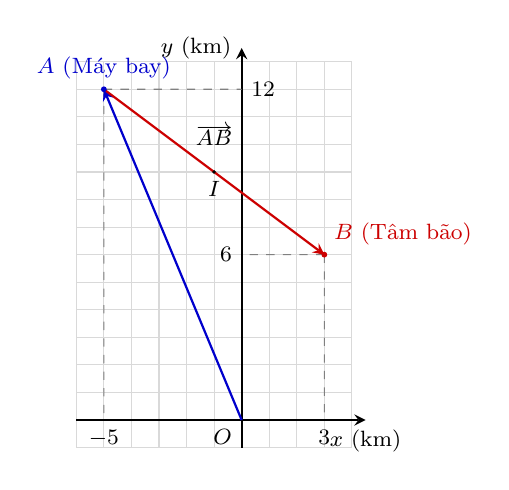
\begin{tikzpicture}[scale=0.35, >=stealth, font=\footnotesize]
		\draw[gray!30, thin, step=1] (-6,-1) grid (4,13);
		\draw[->, thick] (-6,0) -- (4.5,0) node[below]{$x$ (km)};
		\draw[->, thick] (0,-1) -- (0,13.5) node[left]{$y$ (km)};
		\coordinate (O) at (0,0);
		\node[below left] at (O) {$O$};
		\coordinate (A) at (-5, 12);
		\coordinate (B) at (3, 6);
		\coordinate (I) at (-1, 9);
		\draw[dashed, thin, gray] (A) -- (-5,0) node[below, black]{$-5$};
		\draw[dashed, thin, gray] (A) -- (0,12) node[right, black]{$12$};
		\draw[dashed, thin, gray] (B) -- (3,0) node[below, black]{$3$};
		\draw[dashed, thin, gray] (B) -- (0,6) node[left, black]{$6$};
		\draw[->, thick, blue!80!black] (O) -- (A);
		\draw[->, thick, red!80!black] (A) -- (B) node[midway, above, yshift= 2mm , black]{$\overrightarrow{AB}$};
		\fill[blue!80!black] (A) circle (3pt) node[above] {$A$ (Máy bay)};
		\fill[red!80!black] (B) circle (3pt) node[above right] {$B$ (Tâm bão)};
		\fill[black] (I) circle (2pt) node[below] {$I$};
	\end{tikzpicture}
	\end{center}
	\choiceTF
	{\True Vectơ chỉ hướng từ máy bay đến tâm bão là $\overrightarrow{AB} = \left(8; -6\right)$}
	{ Khoảng cách từ máy bay đến tâm bão là $14$ km}
	{\True Nếu máy bay di chuyển thẳng tắp về phía tâm bão và dừng lại ở vị trí trung điểm $I$ của đoạn thẳng $AB$ thì tọa độ của $I$ là $\left(-1; 9\right)$}
	{ Biểu diễn vectơ vị trí của máy bay qua các vectơ đơn vị là $\overrightarrow{OA} = -5\vec{j} + 12\vec{i}$}
\loigiai{
	\begin{itemchoice}
		\itemch Ta có $A(-5; 12)$ và $B(3; 6)$.\\
		Vectơ chỉ hướng từ $A$ đến $B$ là $\overrightarrow{AB} = \left(3 - (-5); 6 - 12\right) = \left(8; -6\right)$.
		\itemch Khoảng cách từ máy bay đến tâm bão là độ dài đoạn thẳng $AB$ là
		$$AB = |\overrightarrow{AB}| = \sqrt{8^2 + (-6)^2} = \sqrt{64 + 36} = \sqrt{100} = 10 \text{ (km)}.$$
		\itemch Tọa độ trung điểm $I$ của đoạn thẳng $AB$ được tính theo công thức:
		$$\heva{&x_I = \dfrac{x_A + x_B}{2} = \dfrac{-5 + 3}{2} = -1 \\&y_I = \dfrac{y_A + y_B}{2} = \dfrac{12 + 6}{2} = 9.}$$
		Vậy $I(-1; 9)$.
		\itemch Vectơ vị trí $\overrightarrow{OA} = \left(-5; 12\right)$.\\
		Biểu diễn qua vectơ đơn vị $\vec{i}$, $\vec{j}$ phải là $\overrightarrow{OA} = -5\vec{i} + 12\vec{j}$.
	\end{itemchoice}
	}
\end{ex}
\Closesolutionfile{ans}
\indapan{3}{ans/ans-vec-to-oxy-ds}
\ind{PHẦN III.} \inden{Câu trả lời ngắn.}
\setcounter{ex}{0}
\Opensolutionfile{ans}[ans/ans-vec-to-oxy-kq]
\begin{ex}%[0H9H1-4]%[Huỳnh Trí Thiện]
	Trong mặt phẳng tọa độ $Oxy$, cho các vectơ $\overrightarrow{a} = \left(2; -1\right)$,  $\overrightarrow{b} = \left(1; 1\right)$ và $\overrightarrow{d} = \left(2m+2; 1-m^2\right)$. Có bao nhiêu giá trị dương của tham số $m$ để $\overrightarrow{d}$ cùng phương với $\overrightarrow{a}$.
	\par
	\shortans[0]{1}
\loigiai{
	Ta có $\overrightarrow{d}$ cùng phương với $\overrightarrow{a}$ khi và chỉ khi $\dfrac{2m+2}{2} = \dfrac{1-m^2}{-1}$
	\[ \Leftrightarrow -2m-2 = 2-2m^2 \Leftrightarrow 2m^2 - 2m - 4 = 0 \Leftrightarrow \hoac{& m=-1 \\& m=2.} \]
	Vì $m$ dương nên $m=2$ thỏa mãn. Vậy có $1$ giá trị.
	}
\end{ex}
\begin{ex}%[0H9H1-4]%[Huỳnh Trí Thiện]
	Trong mặt phẳng tọa độ $Oxy$, cho hai điểm $M\left(5; 3\right)$, $N\left(-3; 5\right)$. Xác định giá trị hoành độ của điểm $P$ sao cho ba điểm $M$, $N$, $P$ thẳng hàng. Biết điểm $P$ nằm trên trục hoành.
	\par
	\shortans{17}
\loigiai{
	$P$ là điểm nằm trên trục hoành nên $P\left(x; 0\right)$.\\
	Ta có $\overrightarrow{MN} = \left(-8; 2\right)$; $\overrightarrow{MP} = \left(x-5; -3\right)$.\\
	Ba điểm $M$, $N$, $P$ thẳng hàng khi $\overrightarrow{MP} = k\overrightarrow{MN} \Leftrightarrow \heva{& x-5 = k \cdot \left(-8\right) \\& -3 = k \cdot 2} \Leftrightarrow \heva{& x=17 \\& k=-\dfrac{3}{2}.}$\\
	Vậy $P\left(17; 0\right) \Rightarrow x_P = 17$.
	}
\end{ex}
\begin{ex}%[0H9V2-1]%[Huỳnh Trí Thiện]
	Trong mặt phẳng tọa độ $Oxy$, cho hai điểm $A\left(1; 5\right)$, $B\left(9; 3\right)$. Có bao nhiêu điểm $M$ thuộc trục hoành thỏa mãn $\widehat{AMB} = 90^\circ$.
	\par
	\shortans{2}
\loigiai{
	Điểm $M$ thuộc trục hoành nên giả sử $M\left(m; 0\right)$.\\
	Ta có $\overrightarrow{MA} = \left(1-m; 5\right)$;  $\overrightarrow{MB} = \left(9-m; 3\right)$.\\
	Theo đề bài, $\widehat{AMB} = 90^\circ \Leftrightarrow \overrightarrow{MA} \cdot \overrightarrow{MB} = 0$
	\[ \Leftrightarrow \left(1-m\right)\left(9-m\right) + 5 \cdot 3 = 0 \Leftrightarrow m^2 - 10m + 24 = 0 \Leftrightarrow \hoac{& m=6 \\& m=4.} \]
	Vậy có $2$ điểm $M$ thỏa mãn yêu cầu bài toán.
	}
\end{ex}
\begin{ex}%[0H9V1-6]%[Huỳnh Trí Thiện]
	Một dòng sông chảy từ phía bắc xuống phía nam với vận tốc là $10\,\text{km/h}$. Một chiếc ca nô chuyển động từ phía đông sang phía tây với vận tốc $40\,\text{km/h}$ so với mặt nước. Tìm vận tốc của ca nô so với bờ sông (\textit{làm tròn kết quả đến hàng phần mười}).
	\shortans{41,2}
	\begin{center}
		% --- CỘT TRÁI: HÌNH VECTƠ ---
		\begin{minipage}[c]{0.65\textwidth}
			\centering
			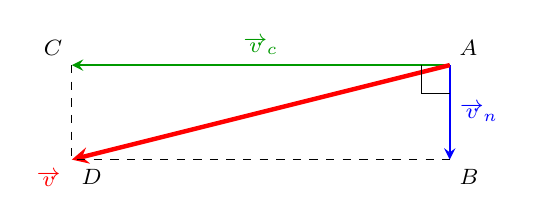
\begin{tikzpicture}[>=stealth, scale=0.12, font=\footnotesize]
				% Định nghĩa tọa độ
				\coordinate (A) at (0,0);
				\coordinate (B) at (0,-10);   % Nước chảy xuống Nam
				\coordinate (C) at (-40,0);   % Ca nô chạy sang Tây
				\coordinate (D) at (-40,-10); % Tổng hợp
				% Vẽ các vectơ
				\draw[->, thick, green!60!black] (A) -- (C) node[midway, above] {$\overrightarrow{v}_c$};
				\draw[->, thick, blue] (A) -- (B) node[midway, right] {$\overrightarrow{v}_n$};
				\draw[->, ultra thick, red] (A) -- (D) node[below left] {$\overrightarrow{v}$};
				% Đường gióng nét đứt
				\draw[dashed] (C) -- (D) -- (B);
				% Kí hiệu vuông góc
				\draw (A) ++(-3,0) -- ++(0,-3) -- ++(3,0);
				% Nhãn điểm
				\node[above right] at (A) {$A$};
				\node[below right] at (B) {$B$};
				\node[above left] at (C) {$C$};
				\node[below right] at (D) {$D$};
			\end{tikzpicture}
		\end{minipage}%
		\hfill % Lệnh đẩy 2 khối minipage ra xa nhau
		% --- CỘT PHẢI: LA BÀN ---
		\begin{minipage}[c]{0.3\textwidth}
			\centering
			\begin{tikzpicture}[>=stealth, scale=0.6, font=\footnotesize]
				% Vẽ trục la bàn
				\draw[<->, gray, thick] (0, 2) node[above]{Bắc} -- (0, -2) node[below]{Nam};
				\draw[<->, gray, thick] (-2, 0) node[left]{Tây} -- (2, 0) node[right]{Đông};
				% Tâm
				\fill[gray] (0,0) circle (1pt);
			\end{tikzpicture}
		\end{minipage}
	\end{center}
	
\loigiai{
	Gọi $\overrightarrow{v}_n$ là vận tốc của dòng nước (chảy từ Bắc xuống Nam), $\left|\overrightarrow{v}_n\right| = 10\,\text{km/h}$.\\
	Gọi $\overrightarrow{v}_c$ là vận tốc của ca nô so với mặt nước (chạy từ Đông sang Tây), $\left|\overrightarrow{v}_c\right| = 40\,\text{km/h}$.\\
	Vận tốc của ca nô so với bờ sông là $\overrightarrow{v} = \overrightarrow{v}_c + \overrightarrow{v}_n$.\\
	Do hướng Bắc - Nam vuông góc với hướng Đông - Tây nên $\overrightarrow{v}_n \perp \overrightarrow{v}_c$.\\
	Theo quy tắc hình bình hành (ở đây là hình chữ nhật), độ lớn của vận tốc tổng hợp là độ dài đường chéo $AD$
	\[ |\overrightarrow{v}| = \sqrt{\left|\overrightarrow{v}_c\right|^2 + \left|\overrightarrow{v}_n\right|^2} = \sqrt{40^2 + 10^2} = \sqrt{1600 + 100} = \sqrt{1700} \approx 41{,}2\,(\text{km/h}). \]
	Vậy vận tốc của ca nô so với bờ sông xấp xỉ $41{,}2\,\text{km/h}$.
	}
\end{ex}
	\begin{ex}%[0H9V1-6]%[Huỳnh Trí Thiện]
	\immini{Để kéo đường dây điện băng qua một hồ hình chữ nhật $ABCD$ với độ dài $AB=140\text{ m}$, $AD=50\text{ m}$. Người ta dự định làm $5$ cột điện liên tiếp thẳng hàng và cách đều nhau. Cột thứ nhất nằm trên bờ $AB$ và cách đỉnh $A$ một khoảng bằng $10\text{ m}$. Cột thứ năm nằm trên bờ $CD$ và cách đỉnh $C$ một khoảng bằng $30\text{ m}$. Khoảng cách từ cột thứ tư đến bờ $AD$ bằng bao nhiêu?
	}{
	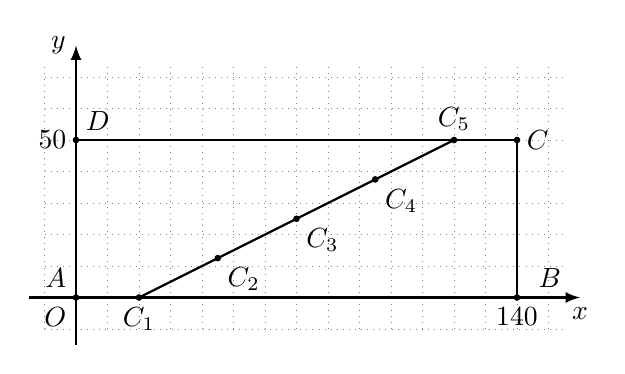
\begin{tikzpicture}[scale=0.8]
		% --- KHU VỰC ĐIỀU CHỈNH TỈ LỆ (SCALE) ---
		% Thay đổi số 1 thành số khác để chỉnh kích thước.
		% Ví dụ: 0.8 (nhỏ hơn), 1.5 (lớn hơn).
		\def\sc{0.5}
		% Thiết lập hệ đơn vị dựa trên biến scale
		% Mặc định 1 đơn vị = 1mm * hệ số scale
		\pgfmathsetmacro{\xscale}{\sc*1mm}
		\pgfmathsetmacro{\yscale}{\sc*1mm}
		% Áp dụng scale vào hệ trục
		\tikzset{x=\xscale, y=\yscale, >=latex}
		% --- Vẽ lưới tọa độ ---
		% Grid step vẫn giữ là 10 đơn vị
		\draw[dotted, help lines, step=10] (-10,-10) grid (155,75);
		% --- Vẽ hệ trục tọa độ ---
		\draw[->, thick] (-15,0) -- (160,0) node[below]{$x$};
		\draw[->, thick] (0,-15) -- (0,80) node[left]{$y$};
		% --- Định nghĩa các điểm ---
		\coordinate (O) at (0,0);
		\coordinate (A) at (0,0);
		\coordinate (B) at (140,0);
		\coordinate (C) at (140,50);
		\coordinate (D) at (0,50);
		% Các điểm trên đoạn thẳng chéo
		\coordinate (C1) at (20,0);
		\coordinate (C5) at (120,50);
		% Các điểm chia đều đoạn thẳng (trung điểm)
		\coordinate (C3) at (70,25);
		\coordinate (C2) at (45,12.5);
		\coordinate (C4) at (95,37.5);
		% --- Vẽ các đường ---
		\draw[thick] (D) -- (C) -- (B);
		\draw[thick] (A) -- (B);
		\draw[thick] (A) -- (D);
		\draw[thick] (C1) -- (C5);
		% --- Vẽ các điểm tròn ---
		% Kích thước điểm cũng được điều chỉnh nhẹ theo scale để không bị quá bé hoặc quá to
		\foreach \p in {A,B,C,D,C1,C2,C3,C4,C5}
		\fill (\p) circle (1.5pt);
		% --- Ghi chú (Labels) ---
		\node[above left] at (A) {$A$};
		\node[below left] at (O) {$O$};
		\node[left] at (0,50) {$50$};
		\node[above right, xshift=0 mm] at (D) {$D$};
		\node[below] at (B) {$140$};
		\node[above right, xshift=1.5mm] at (B) {$B$};
		\node[right] at (C) {$C$};
		\node[below] at (C1) {$C_1$};
		\node[below right] at (C2) {$C_2$};
		\node[below right] at (C3) {$C_3$};
		\node[below right] at (C4) {$C_4$};
		\node[above] at (C5) {$C_5$};
	\end{tikzpicture}
	}	\par
	\shortans{85}
\loigiai{
	Chọn hệ trục tọa độ $Oxy$ sao cho $A\left(0; 0\right)$, $B\left(140; 0\right)$, $D\left(0; 50\right)$.\\
	Khi đó $C\left(140; 50\right)$.\\
	Gọi vị trí $5$ cột điện là $C_1, C_2, C_3, C_4, C_5$.\\
	Theo đề bài, cột thứ nhất $C_1$ nằm trên $AB$ và cách $A$ một khoảng $10\text{ m}$ nên $C_1\left(10; 0\right)$.\\
	Cột thứ năm $C_5$ nằm trên $CD$ và cách $C$ một khoảng $30\text{ m}$ nên $x_{C_5} = 140 - 30 = 110$.\\
	Do đó $C_5\left(110; 50\right)$.\\
	Ta có $\overrightarrow{C_1C_5} = \left(100; 50\right)$.\\
	Vì $5$ cột điện thẳng hàng và cách đều nhau nên ta có
	\[ \overrightarrow{C_1C_4} = \dfrac{3}{4}\overrightarrow{C_1C_5} = \dfrac{3}{4}\left(100; 50\right) = \left(75; \dfrac{75}{2}\right). \]
	Suy ra tọa độ điểm $C_4$ là
	\[ \heva{x_{C_4} &= 10 + 75 = 85 \\ y_{C_4} &= 0 + \dfrac{75}{2} = \dfrac{75}{2}.} \Rightarrow C_4\left(85; 37{,}5\right). \]
	Khoảng cách từ cột thứ tư ($C_4$) đến bờ $AD$ (trục tung $Oy$) chính là hoành độ của điểm $C_4$.\\
	Vậy khoảng cách cần tìm là $85\text{ m}$.
	}
\end{ex}
	\begin{ex}%[0H9C1-6]%[Huỳnh Trí Thiện]
	\immini{	Một con lắc đơn đang đứng yên tại vị trí cân bằng $M$ thì được tác dụng một lực $\overrightarrow{F}$ để đưa đến vị trí $I$ và giữ yên (như hình vẽ). Biết rằng con lắc đang chịu tác dụng của lực căng dây $\overrightarrow{T}$ có cường độ $30\,\text{N}$, trọng lực $\overrightarrow{P}$ và lực tác dụng $\overrightarrow{F}$ theo phương ngang. Hãy xác định cường độ của lực $\overrightarrow{F}$.
	}{
	\begin{tikzpicture}[>=Stealth, scale=0.8, font=\fontsize{10}{10}\selectfont]
		% --- ĐỊNH NGHĨA THÔNG SỐ ---
		\def\length{4.5}   % Chiều dài dây
		\def\angle{35}     % Góc lệch alpha
		\coordinate (O) at (0,0); % Điểm treo
		\coordinate (M) at (0,-\length); % Vị trí cân bằng (trên dây)
		\coordinate (I) at ({\length*sin(\angle)},{-\length*cos(\angle)}); % Vị trí I
		% --- VẼ TRẦN VÀ ĐIỂM TREO ---
		% Phần gạch chéo (trần)
		\fill[pattern=north east lines, pattern color=black] (-1,0) rectangle (1,0.3);
		\draw[thick] (-1,0) -- (1,0); % Đường trần
		\node[left] at (-0.2, -0.3) {Điểm treo};
		% --- VẼ ĐƯỜNG DÓNG VÀ QUỸ ĐẠO ---
		% Đường thẳng đứng đứt nét (trục thẳng đứng)
		\draw[dashed, thick] (O) -- (0, -\length - 1);
		% Điểm M và nhãn
		\fill (M) circle (2pt);
		\node[left] at (M) {Vị trí cân bằng $M$};
		% Cung tròn đứt nét (quỹ đạo từ M đến I)
		\draw[dashed] (M) arc (-90:-90+\angle:\length);
		% --- VẼ DÂY VÀ GÓC ---
		% Dây treo
		\draw[thick] (O) -- (I);
		% Kí hiệu góc alpha
		\draw[thick] (0,-1) arc (-90:-90+\angle:1);
		\node at ({(\angle/2)-90}:1.3) {$\alpha$};
		% --- VẼ VẬT (QUẢ CẦU) ---
		\shade[ball color=gray!50] (I) circle (0.35);
		\node[above right] at ($(I)+(0,0.3)$) {Vị trí $I$};
		% --- CÁC VECTƠ LỰC (QUAN TRỌNG) ---
		% 1. Lực căng dây T (Màu xanh lá đậm)
		% Vẽ từ tâm I hướng về điểm treo O
		\draw[->, line width=1.5pt, color=green!60!black] (I) -- ($(I)!0.45!(O)$)
		node[right, black] {$\overrightarrow{T}$ (Lực căng dây)};
		% 2. Lực tác dụng F (Màu xanh dương)
		% Vẽ từ tâm I hướng sang ngang
		\draw[->, line width=1.5pt, color=cyan!80!blue] (I) -- ++(2,0)
		node[right, black] {$\overrightarrow{F}$ (Lực tác dụng)};
		% 3. Trọng lực P (Màu đỏ)
		% Vẽ từ tâm I hướng thẳng đứng xuống dưới
		\draw[->, line width=1.5pt, color=red] (I) -- ++(0,-2)
		node[right, black] {$\overrightarrow{P}$ (Trọng lực)};
	\end{tikzpicture}
	}	\par
	\shortans{15}
\loigiai{
	Con lắc chịu tác dụng của ba lực: trọng lực $\overrightarrow{P}$, lực căng dây $\overrightarrow{T}$ và lực kéo $\overrightarrow{F}$.\\
	Khi con lắc nằm cân bằng tại vị trí $I$, tổng hợp lực tác dụng lên vật bằng $\vec{0}$
	\[ \overrightarrow{P} + \overrightarrow{F} + \overrightarrow{T} = \vec{0} \Rightarrow \overrightarrow{P} + \overrightarrow{F} = -\overrightarrow{T}. \]
	Điều này có nghĩa là hợp lực của $\overrightarrow{P}$ và $\overrightarrow{F}$ phải cân bằng với lực căng dây $\overrightarrow{T}$.\\
	Ta có sơ đồ vectơ lực tạo thành một tam giác vuông (do $\overrightarrow{P}$ thẳng đứng vuông góc với $\overrightarrow{F}$ nằm ngang). Trong tam giác vuông này
	\begin{itemize}
		\item Cạnh huyền tương ứng với độ lớn của lực căng dây $|\overrightarrow{T}| = 30\,\text{N}$.
		\item Cạnh đối diện với góc lệch $30^\circ$ (góc ở đỉnh tam giác lực, bằng góc lệch dây treo so le trong) tương ứng với độ lớn của lực $\overrightarrow{F}$.
	\end{itemize}
	Dựa vào hệ thức lượng trong tam giác vuông
	\[ \sin 30^\circ = \dfrac{|\overrightarrow{F}|}{|\overrightarrow{T}|} \Rightarrow |\overrightarrow{F}| = |\overrightarrow{T}| \cdot \sin 30^\circ=30 \cdot \dfrac{1}{2} = 15\,\text{N}. \]
	Vậy cường độ của lực $\overrightarrow{F}$ là $15\,\text{N}$.
	}
\end{ex}
\Closesolutionfile{ans}
\indapan{4}{ans/ans-vec-to-oxy-kq}
\ind{PHẦN IV.} \inden{Tự luận.}
\setcounter{ex}{0}
% --- Bài 2 ---
\begin{ex}%[0H9H1-2]
	Tìm tọa độ của vectơ $\overrightarrow{u}$ biết
	\begin{enumerate}[a)]
		\item $\overrightarrow{u} + 3\overrightarrow{a} = 4\overrightarrow{b}$ với $\overrightarrow{a} = \left(2; -3\right)$ và $\overrightarrow{b} = \left(-25; 5\right)$.
		\item $2\overrightarrow{u} - 5\overrightarrow{a} = 3\overrightarrow{b}$ với $\overrightarrow{a} = \left(-3; 7\right)$ và $\overrightarrow{b} = \left(-6; -7\right)$.
	\end{enumerate}
\loigiai{
	a) Ta có $\overrightarrow{u} + 3\overrightarrow{a} = 4\overrightarrow{b} \Rightarrow \overrightarrow{u} = 4\overrightarrow{b} - 3\overrightarrow{a}$.\\
	Với $\overrightarrow{a} = \left(2; -3\right) \Rightarrow 3\overrightarrow{a} = \left(6; -9\right)$.\\
	Với $\overrightarrow{b} = \left(-25; 5\right) \Rightarrow 4\overrightarrow{b} = \left(-100; 20\right)$.\\
	Suy ra $\overrightarrow{u} = \left(-100 - 6; 20 - (-9)\right) = \left(-106; 29\right)$.\\
	Vậy $\overrightarrow{u} = \left(-106; 29\right)$.
	b) Ta có $2\overrightarrow{u} - 5\overrightarrow{a} = 3\overrightarrow{b} \Rightarrow 2\overrightarrow{u} = 3\overrightarrow{b} + 5\overrightarrow{a}$.\\
	Với $\overrightarrow{a} = \left(-3; 7\right) \Rightarrow 5\overrightarrow{a} = \left(-15; 35\right)$.\\
	Với $\overrightarrow{b} = \left(-6; -7\right) \Rightarrow 3\overrightarrow{b} = \left(-18; -21\right)$.\\
	Suy ra $2\overrightarrow{u} = \left(-18 + (-15); -21 + 35\right) = \left(-33; 14\right)$.\\
	Do đó $\overrightarrow{u} = \left(-\dfrac{33}{2}; 7\right)$.
	}
\end{ex}
% --- Bài 3 ---
\begin{ex}%[0H9H1-3]
	Cho $3$ điểm $A\left(2; 5\right)$, $B\left(1; 1\right)$, $C\left(3; 3\right)$.
	\begin{enumerate}
		\item Tìm tọa độ điểm $D$ sao cho $\overrightarrow{AD} = 3\overrightarrow{AB} - 2\overrightarrow{AC}$.
		\item Tìm tọa độ điểm $N$ sao cho $\overrightarrow{AN} + 2\overrightarrow{AB} - 3\overrightarrow{CN} = \overrightarrow{0}$.
	\end{enumerate}
\loigiai{
	Ta có $\overrightarrow{AB} = \left(1 - 2; 1 - 5\right) = \left(-1; -4\right)$.\\
	Ta có $\overrightarrow{AC} = \left(3 - 2; 3 - 5\right) = \left(1; -2\right)$.
	\begin{enumerate}[a)]
		\item Gọi $D\left(x; y\right)$, ta có $\overrightarrow{AD} = \left(x - 2; y - 5\right)$.\\
		Ta có $3\overrightarrow{AB} = \left(-3; -12\right)$ và $2\overrightarrow{AC} = \left(2; -4\right)$.\\
		Theo đề bài $\overrightarrow{AD} = 3\overrightarrow{AB} - 2\overrightarrow{AC}$ $$\Rightarrow \heva{&x - 2 = -3 - 2 \\&y - 5 = -12 - (-4)} \Leftrightarrow \heva{x - 2 = -5 \\ y - 5 = -8} \Leftrightarrow \heva{x = -3 \\ y = -3.}$$\\
		Vậy $D\left(-3; -3\right)$.
		\item Gọi $N\left(x; y\right)$. Khi đó $\overrightarrow{AN} = \left(x - 2; y - 5\right)$ và $\overrightarrow{CN} = \left(x - 3; y - 3\right)$.\\
		Ta có $\overrightarrow{AN} + 2\overrightarrow{AB} - 3\overrightarrow{CN} = \overrightarrow{0}$
		$$ \Rightarrow \heva{&(x - 2) + 2(-1) - 3(x - 3) = 0 \\&(y - 5) + 2(-4) - 3(y - 3) = 0}\\
		\Leftrightarrow \heva{x - 2 - 2 - 3x + 9 = 0 \\ y - 5 - 8 - 3y + 9 = 0} \Leftrightarrow \heva{-2x + 5 = 0 \\ -2y - 4 = 0} \Leftrightarrow \heva{x = \dfrac{5}{2} \\ y = -2.}$$
		Vậy $N\left(\dfrac{5}{2}; -2\right)$.
	\end{enumerate}
	}
\end{ex}
\begin{ex}%[0H9V1-6]%[Huỳnh Trí Thiện]
	\immini{Hai máy tời kéo tàu biển được đặt ở hai vị trí $B$, $D$ dọc theo kênh đào được minh họa ở hình dưới đây. Hai máy tời đó kéo một con tàu từ vị trí $A$ hướng đến vị trí $C$. Biết tọa độ các điểm $A\left(\dfrac{13}{2};8\right)$, $B\left(3;7\right)$, $D\left(6;4\right)$. Biết điểm $C\left(a;b\right)$, tính giá trị của biểu thức $a+b$.}{
	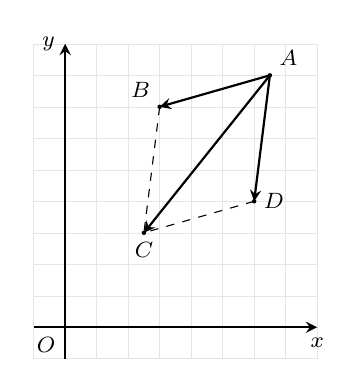
\begin{tikzpicture}[scale=0.4, >=stealth, font=\footnotesize]
		% --- Lưới tọa độ ---
		\draw[step=1, gray!20, very thin] (-1,-1) grid (8,9);
		% --- Hệ trục ---
		\draw[->, thick] (-1,0) -- (8,0) node[below]{$x$};
		\draw[->, thick] (0,-1) -- (0,9) node[left]{$y$};
		\node[below left] at (0,0) {$O$};
		% --- Các điểm ---
		\coordinate (A) at (6.5, 8);
		\coordinate (B) at (3, 7);
		\coordinate (D) at (6, 4);
		% Tính toán điểm C = A + AB + AD
		% AB = (-3.5, -1), AD = (-0.5, -4) => AC = (-4, -5) => C = (2.5, 3)
		\coordinate (C) at (2.5, 3);
		% --- Vẽ vectơ và đoạn thẳng ---
		\draw[->, thick] (A) -- (B);
		\draw[->, thick] (A) -- (D);
		\draw[->, thick] (A) -- (C); % Vectơ tổng hợp
		\draw[dashed] (B) -- (C);
		\draw[dashed] (D) -- (C);
		% --- Điểm và Nhãn ---
		\fill (A) circle (2pt) node[above right] {$A$};
		\fill (B) circle (2pt) node[above left] {$B$};
		\fill (C) circle (2pt) node[below] {$C$};
		\fill (D) circle (2pt) node[right] {$D$};
	\end{tikzpicture}
	}
\loigiai{
	Ta có $\overrightarrow{AB} = \left(3 - \dfrac{13}{2}; 7 - 8\right) = \left(-\dfrac{7}{2}; -1\right)$.\\
	Ta có $\overrightarrow{AD} = \left(6 - \dfrac{13}{2}; 4 - 8\right) = \left(-\dfrac{1}{2}; -4\right)$.\\
	Mặt khác tàu di chuyển từ $A$ đến $C$ dưới tác động kéo của hai máy tời nên theo quy tắc hình bình hành ta có
	\[ \overrightarrow{AC} = \overrightarrow{AB} + \overrightarrow{AD} \Rightarrow \overrightarrow{AC} = \left(-\dfrac{7}{2} - \dfrac{1}{2}; -1 - 4\right) = \left(-4; -5\right). \]
	Gọi $C\left(a; b\right)$, khi đó $\overrightarrow{AC} = \left(a - \dfrac{13}{2}; b - 8\right)$.\\
	Suy ra
	\[ \heva{&a - \dfrac{13}{2} = -4 \\&b - 8 = -5} \Leftrightarrow \heva{&a = -4 + \dfrac{13}{2} \\&b = 3} \Leftrightarrow \heva{&a = \dfrac{5}{2} \\&b = 3.} \]
	Vậy $a + b = \dfrac{5}{2} + 3 = \dfrac{11}{2} = 5{,}5$.
	}
\end{ex}
\begin{ex}%[0H9V1-6]%[Huỳnh Trí Thiện]
	Trên màn hình ra đa, đài kiểm soát không lưu được đặt tại gốc tọa độ $O\left(0;0\right)$. Một máy bay trực thăng xuất phát từ sân bay $A$ có tọa độ $\left(-20; 10\right)$ chuyển động thẳng đều với vận tốc được biểu diễn bởi vectơ $\overrightarrow{v_A} = \left(40; 10\right)$ (đơn vị $\text{km/h}$). Cùng lúc đó, một máy bay vận tải khác xuất phát từ sân bay $B$ có tọa độ $\left(10; 80\right)$ bay theo đường thẳng với vận tốc không đổi để gặp máy bay trực thăng sau $2$ giờ bay.
	\begin{enumerate}[a)]
		\item Xác định tọa độ vị trí gặp nhau của hai máy bay.
		\item Tìm tọa độ vectơ vận tốc $\overrightarrow{v_B}$ của máy bay vận tải và tính tốc độ của nó.\\(\textit{Kết quả làm tròn đến hàng đơn vị}).
	\end{enumerate}
\loigiai{
	\immini{
	\begin{enumerate}[a)]
		\item Gọi $M\left(x;y\right)$ là vị trí gặp nhau của hai máy bay sau $t=2$ giờ.\\
		Vị trí của máy bay trực thăng sau $2$ giờ là
		\[ \heva{&x_M = x_A + 2 \cdot v_{Ax} \\&y_M = y_A + 2 \cdot v_{Ay} }. \Leftrightarrow \heva{&x_M= -20 + 2 \cdot 40 = 60 \\&y_M= 10 + 2 \cdot 10 = 30}\]
		Vậy tọa độ điểm gặp nhau là $M\left(60; 30\right)$.\\
		\item Trong $2$ giờ, máy bay vận tải di chuyển từ $B\left(10; 80\right)$ đến $M\left(60; 30\right)$.\\
		Vectơ độ dời của máy bay vận tải là $\overrightarrow{BM} = \left(60 - 10; 30 - 80\right) = \left(50; -50\right)$.\\
		Vì thời gian bay là $2$ giờ nên vectơ vận tốc $\overrightarrow{v_B}$ là
		\[ \overrightarrow{v_B} = \dfrac{1}{2}\overrightarrow{BM} = \dfrac{1}{2}\left(50; -50\right) = \left(25; -25\right). \]
		Tốc độ của máy bay vận tải là độ lớn của vectơ $\overrightarrow{v_B}$
		\[ |\overrightarrow{v_B}| = \sqrt{25^2 + \left(-25\right)^2} = \sqrt{625 + 625} = \sqrt{1250} \approx 35\,(\text{km/h}). \]
	\end{enumerate}
	}{
	\begin{tikzpicture}[scale=0.06, >=stealth, font=\footnotesize]
		% Lưới và trục
		\draw[gray!20, step=10] (-30,-10) grid (70,90);
		\draw[->] (-35,0) -- (75,0) node[below]{$x$};
		\draw[->] (0,-15) -- (0,95) node[left]{$y$};
		\node[below left] at (0,0) {$O$};
		% Tọa độ
		\coordinate (A) at (-20,10);
		\coordinate (B) at (10,80);
		\coordinate (M) at (60,30); % Điểm gặp nhau
		% Đường bay
		\draw[->, thick, blue] (A) -- (M) node[midway, below right] {Trực thăng};
		\draw[->, thick, red] (B) -- (M) node[midway, above right] {Vận tải};
		% Điểm
		\fill (A) circle (20pt) node[below] {$A$};
		\fill (B) circle (20pt) node[above] {$B$};
		\fill (M) circle (20pt) node[right] {$M$ (Gặp nhau)};
		% Gióng tọa độ M
		\draw[dashed, gray] (M) -- (60,0) node[below, black]{$60$};
		\draw[dashed, gray] (M) -- (0,30) node[left, black]{$30$};
	\end{tikzpicture}
	}
	}
\end{ex}
\begin{ex}%[0H9V1-6]%[Huỳnh Trí Thiện]
	\immini{Để kéo đường dây điện băng qua một hồ hình chữ nhật $ABCD$ với độ dài $AB=200\,\text{m}$, $AD=180\,\text{m}$, người ta dự định làm $4$ cột điện liên tiếp cách đều. Cột thứ nhất nằm trên bờ $AB$ và cách đỉnh $A$ khoảng cách $20\,\text{m}$, cột thứ tư nằm trên bờ $CD$ và cách đỉnh $C$ khoảng cách $30\,\text{m}$. Tính các khoảng cách từ vị trí các cột thứ hai, thứ ba đến các bờ $AB$, $AD$.
	}{
	\begin{tikzpicture}[scale=0.015, >=stealth, font=\footnotesize]
		% --- Lưới tọa độ ---
		\draw[step=20, gray!20, very thin] (-10,-10) grid (230,210);
		% --- Hệ trục ---
		\draw[->] (-20,0) -- (240,0) node[below]{$x$};
		\draw[->] (0,-20) -- (0,220) node[left]{$y$};
		% --- Hình chữ nhật ABCD ---
		\coordinate (A) at (0,0);
		\coordinate (B) at (200,0);
		\coordinate (C) at (200,180);
		\coordinate (D) at (0,180);
		\draw[thick] (A) -- (B) node[below]{$200$} -- (C) -- (D) node[left]{$180$} -- cycle;
		% --- Các điểm cột điện ---
		\coordinate (C1) at (20,0);
		% C4 cách C 30m, C có x=200 => C4 có x=170
		\coordinate (C4) at (170,180);
		% Tính toán C2, C3 chia đoạn C1C4 thành 3 phần
		\coordinate (C2) at ($(C1)!1/3!(C4)$);
		\coordinate (C3) at ($(C1)!2/3!(C4)$);
		% --- Vẽ dây điện ---
		\draw[thick] (C1) -- (C4);
		% --- Đường gióng đứt đoạn ---
		% Gióng C2
		\draw[dashed, blue] (C2) -- (C2|-A) node[below, blue]{$70$};
		\draw[dashed, blue] (C2) -- (C2-|A) node[left, blue]{$60$};
		% Gióng C3
		\draw[dashed, blue] (C3) -- (C3|-A); % node[below]{120};
		\draw[dashed, blue] (C3) -- (C3-|A); % node[left]{120};
		% --- Các điểm và nhãn ---
		\node[below left] at (A) {$A$};
		\node[above right] at (B) {$B$};
		\node[above right] at (C) {$C$};
		\node[above right] at (D) {$D$};
		\fill (C1) circle (100pt) node[below, yshift=-3mm] {$C_1$};
		\fill (C2) circle (100pt) node[above left, xshift=-2mm] {$C_2$};
		\fill (C3) circle (100pt) node[above left] {$C_3$};
		\fill (C4) circle (100pt) node[above] {$C_4$};
	\end{tikzpicture}
	}
\loigiai{
	Chọn hệ trục tọa độ $Oxy$ sao cho $A(0;0)$, $B(200;0)$, $D(0;180)$. Khi đó $C(200;180)$.\\
	Vị trí các cột điện được trồng là $C_1$,  $C_2$, $C_3$, $C_4$.\\
	Theo giả thiết
	\begin{itemize}
		\item $C_1$ thuộc cạnh $AB$ và $AC_1 = 20 \Rightarrow C_1(20;0)$.
		\item $C_4$ thuộc cạnh $CD$ và $C_4C = 30$. Vì $C$ có hoành độ $200$ nên $C_4$ có hoành độ $200-30=170$. Tung độ của $C_4$ bằng tung độ của $C$ và $D$ là $180$. Vậy $C_4(170;180)$.
	\end{itemize}
	Ta có $\overrightarrow{C_1C_4} = (170-20; 180-0) = (150; 180)$.\\
	Vì bốn cột điện được trồng liên tiếp, cách đều thẳng hàng nên $C_1C_2 = C_2C_3 = C_3C_4 = \dfrac{1}{3}C_1C_4$.\\
	Suy ra $\overrightarrow{C_1C_2} = \dfrac{1}{3}\overrightarrow{C_1C_4} = \dfrac{1}{3}(150; 180) = (50; 60)$.\\
	Giả sử $C_2(x_2; y_2)$, ta có $\overrightarrow{C_1C_2} = (x_2-20; y_2-0)$.\\
	Từ đó suy ra $\heva{x_2-20 = 50 \\ y_2 = 60} \Leftrightarrow \heva{x_2 = 70 \\ y_2 = 60}$. \\ Vậy $C_2(70; 60)$.\\
	Tương tự, $\overrightarrow{C_1C_3} = \dfrac{2}{3}\overrightarrow{C_1C_4} = (100; 120) \Rightarrow C_3(120; 120)$.\\
	Khoảng cách từ $C_2$ đến bờ $AB$ là $y_2 = 60\,\text{m}$, đến bờ $AD$ là $x_2 = 70\,\text{m}$.\\
	Khoảng cách từ $C_3$ đến bờ $AB$ là $y_3 = 120\,\text{m}$, đến bờ $AD$ là $x_3 = 120\,\text{m}$.
	}
\end{ex}
\begin{ex}%[0H9C1-6]%[Huỳnh Trí Thiện]
	\immini{Một đèn chùm trang trí có trọng lượng $P = 100\,\text{N}$ được treo cố định vào trần nhà bởi hai sợi dây cáp $AC$ và $BC$ như hình vẽ (điểm $C$ là vị trí treo đèn). Trong mặt phẳng tọa độ $Oxy$ (trục $Oy$ thẳng đứng hướng lên), lực căng của dây $AC$ được biểu diễn bởi vectơ $\overrightarrow{T_1} = \left(-60; 80\right)$ (đơn vị Newton). Để đèn nằm cân bằng (tổng hợp lực tại $C$ bằng $\overrightarrow{0}$), hãy xác định tọa độ và độ lớn của vectơ lực căng $\overrightarrow{T_2}$ trên dây $BC$, biết rằng trọng lực $\overrightarrow{P}$ có hướng thẳng đứng xuống dưới và có tọa độ là $\left(0; -100\right)$.(\textit{Kết quả làm tròn đến hàng phần mười})
	}{
	\begin{tikzpicture}[scale=0.03, >=stealth, font=\small]
		% --- 1. CẤU TRÚC TRẦN VÀ DÂY (Minh họa thực tế) ---
		\def\ceilH{90} % Độ cao trần
		% Trần nhà (Họa tiết)
		\fill[pattern=north east lines, pattern color=gray!30] (-80,\ceilH) rectangle (80,\ceilH+4);
		\draw[thick] (-80,\ceilH) -- (80,\ceilH);
		\node[fill=white, inner sep=1pt] at (0,\ceilH) [above right=2mm] {Trần nhà};
		% Điểm treo trên trần (Tính toán giao điểm)
		% Dây trái theo hướng T1(-60,80) -> y = -4/3 x. Tại y=90 -> x = -67.5
		\coordinate (WallLeft) at (-67.5, \ceilH);
		% Dây phải theo hướng T2(60,20) -> y = 1/3 x. Tại y=90 -> x = 270 (Rất xa)
		% Ta lấy điểm trên biên hình vẽ để vẽ dây phải
		\coordinate (WallRight) at (80, 26.66);
		% Vẽ 2 dây cáp (Nét kép cho giống dây cáp)
		\draw[double, double distance=1pt, line width=1pt, gray] (0,0) -- (WallLeft);
		\draw[double, double distance=1pt, line width=1pt, gray] (0,0) -- (WallRight);
		% Móc treo tại C
		\fill[gray!50!black] (0,0) circle (1.5);
		% --- 2. VẼ ĐÈN CHÙM (Trang trí cổ điển) ---
		\begin{scope}[yshift=0cm]
			% Xích treo đèn
			\draw[thick, double, gray!80!black] (0,0) -- (0,-15);
			% Thân đèn chính
			\shade[ball color=orange!30!brown] (0,-20) circle (6);
			\draw[thick, orange!20!brown, fill=orange!10] (-20,-15) .. controls (-10,-35) and (10,-35) .. (20,-15) -- cycle;
			\draw[thick, brown] (-20,-15) -- (20,-15);
			% Các bóng đèn/nhánh đèn
			\foreach \x in {-18, -9, 9, 18} {
			\draw[thick, brown] (\x, -15) -- (\x, -10);
			\shade[ball color=yellow!20] (\x, -8) ellipse (2 and 3);
			}
			% Đáy đèn
			\draw[thick, brown] (0,-25) -- (0,-35);
			\shade[ball color=orange!30!brown] (0,-38) circle (3);
		\end{scope}
		% --- 3. HỆ TRỤC VÀ VECTƠ LỰC (Lớp toán học) ---
		\draw[->, gray!60] (-70,0) -- (70,0) node[below]{$x$};
		\draw[->, gray!60] (0,-80) -- (0,100) node[left]{$y$};
		\node[above right, xshift=0.6mm, yshift=1.5mm , gray] at (0,0) {$O(C)$};
		% Định nghĩa các điểm mút vectơ
		\coordinate (O) at (0,0);
		\coordinate (T1) at (-60,80);
		\coordinate (T2) at (60,20);
		\coordinate (P) at (0,-80);
		% Vẽ các vectơ
		\draw[->, line width=1.2pt, blue] (O) -- (T1) node[midway, above left, sloped] {$\overrightarrow{T_1}$};
		\draw[->, line width=1.2pt, red] (O) -- (P) node[right, near end] {$\overrightarrow{P}$};
		\draw[->, line width=1.2pt, green!50!black] (O) -- (T2) node[midway, below right, sloped] {$\overrightarrow{T_2}$};
		% Đường gióng tọa độ (nét đứt)
		\draw[dashed, thin, blue] (T1) -- (-60,0) node[below]{$-60$};
		\draw[dashed, thin, blue] (T1) -- (0,80) node[right]{$80$};
		\draw[dashed, thin, green!50!black] (T2) -- (60,0) node[below]{$60$};
		\draw[dashed, thin, green!50!black] (T2) -- (0,20) node[left]{$20$};
		\node[right, red] at (0,-80) {$-100$};
	\end{tikzpicture}
	}
\loigiai{
	Để đèn nằm cân bằng, tổng hợp lực tác dụng lên điểm treo $C$ phải bằng $\overrightarrow{0}$
	\[ \overrightarrow{T_1} + \overrightarrow{T_2} + \overrightarrow{P} = \overrightarrow{0} \Rightarrow \overrightarrow{T_2} = -\left(\overrightarrow{T_1} + \overrightarrow{P}\right). \]
	Ta có $\overrightarrow{T_1} = \left(-60; 80\right)$ và $\overrightarrow{P} = \left(0; -100\right)$.\\
	Tổng hợp $\overrightarrow{T_1} + \overrightarrow{P} = \left(-60 + 0; 80 - 100\right) = \left(-60; -20\right)$.\\
	Suy ra $\overrightarrow{T_2} = -\left(-60; -20\right) = \left(60; 20\right)$.\\
	Độ lớn của lực căng dây $BC$ là
	\[ |\overrightarrow{T_2}| = \sqrt{60^2 + 20^2} = \sqrt{3600 + 400} = \sqrt{4000} \approx 63{,}2\,(\text{N}). \]
	Vậy $\overrightarrow{T_2} = \left(60; 20\right)$ và độ lớn khoảng $63{,}2\,\text{N}$.
	}
\end{ex}